% !TeX program = pdflatex
%==============================================================================
%  MagicFrens "Cauldron" --- Independent Security Audit (September 2026)
%
%  This is a NEW, from-scratch review. It was derived exclusively from the
%  Solidity sources under contracts/solidity/ and from the test suite read as
%  evidence of intended behaviour. No pre-existing audit, report, exploit
%  write-up, design document or runbook in this repository was opened while it
%  was produced, and no prior finding tag was consulted or reused. Where a
%  conclusion coincides with earlier work, it was re-derived here.
%
%  Build:  pdflatex MagicFrens_Independent_Audit_2026-09.tex   (x3, for the TOC)
%     or:  tectonic MagicFrens_Independent_Audit_2026-09.tex
%==============================================================================
\documentclass[11pt,a4paper]{article}

\usepackage[T1]{fontenc}
\usepackage[utf8]{inputenc}
\usepackage[margin=2.4cm]{geometry}
\usepackage{booktabs}
\usepackage{longtable}
\usepackage{array}
\usepackage{xcolor}
\usepackage{colortbl}
\usepackage{fancyhdr}
\usepackage{titlesec}
\usepackage{enumitem}
\usepackage{listings}
\usepackage{tikz}
\usetikzlibrary{arrows.meta,positioning,shapes.geometric,fit,backgrounds}
\usepackage[hidelinks,bookmarks=true]{hyperref}
\usepackage{amssymb}
\usepackage{amsmath}
\usepackage{tcolorbox}
\tcbuselibrary{breakable,skins}

%------------------------------------------------------------------ palette ---
\definecolor{ink}{HTML}{16181D}
\definecolor{slate}{HTML}{5B6472}
\definecolor{rule}{HTML}{D5D9E0}
\definecolor{critical}{HTML}{9B1C1C}
\definecolor{high}{HTML}{C2410C}
\definecolor{medium}{HTML}{A16207}
\definecolor{low}{HTML}{1D4ED8}
\definecolor{info}{HTML}{4B5563}
\definecolor{good}{HTML}{15803D}
\definecolor{panel}{HTML}{F6F7F9}

\hypersetup{colorlinks=false}

%----------------------------------------------------------------- typography -
\titleformat{\section}{\Large\bfseries\color{ink}\raggedright}{\thesection}{0.7em}{}
\titleformat{\subsection}{\normalsize\bfseries\color{ink}\raggedright}{\thesubsection}{0.6em}{}
\titleformat{\subsubsection}{\normalsize\bfseries\color{ink}}{\thesubsubsection}{0.5em}{}
\setlist{leftmargin=1.35em,itemsep=2pt,topsep=3pt}

\pagestyle{fancy}\fancyhf{}
\fancyhead[L]{\small\color{slate}MagicFrens Cauldron --- Independent Security Audit}
\fancyhead[R]{\small\color{slate}\thepage}
\renewcommand{\headrulewidth}{0.4pt}

\lstdefinestyle{sol}{
  basicstyle=\ttfamily\scriptsize,
  breaklines=true,
  columns=fullflexible,
  keywordstyle=\color{low},
  commentstyle=\color{slate}\itshape,
  stringstyle=\color{good},
  numbers=none,
  frame=leftline,
  framerule=1.5pt,
  rulecolor=\color{rule},
  xleftmargin=0.9em,
  showstringspaces=false,
  language=Java,
}
\lstset{style=sol}

%------------------------------------------------------------------- macros ---
\newcommand{\SevCrit}{\textcolor{critical}{\textbf{Critical}}}
\newcommand{\SevHigh}{\textcolor{high}{\textbf{High}}}
\newcommand{\SevMed}{\textcolor{medium}{\textbf{Medium}}}
\newcommand{\SevLow}{\textcolor{low}{\textbf{Low}}}
\newcommand{\SevInfo}{\textcolor{info}{\textbf{Info}}}
\newcommand{\Conf}{\textcolor{critical}{Confirmed}}
\newcommand{\Susp}{\textcolor{medium}{Suspected}}
\newcommand{\Refu}{\textcolor{good}{Refuted}}
\newcommand{\code}[1]{\texttt{\small #1}}
\newcommand{\fileref}[1]{\texttt{\scriptsize #1}}

\newtcolorbox{findingbox}[2]{
  breakable, enhanced, colback=panel, colframe=#1, boxrule=0.9pt,
  left=6pt,right=6pt,top=5pt,bottom=5pt, arc=1pt,
  title={#2}, fonttitle=\bfseries\small\color{white}, coltitle=white
}
\newtcolorbox{notebox}[1]{
  breakable, enhanced, colback=panel, colframe=rule, boxrule=0.7pt,
  left=6pt,right=6pt,top=5pt,bottom=5pt, arc=1pt,
  title={#1}, fonttitle=\bfseries\small\color{ink}, coltitle=ink
}

\sloppy
\begin{document}

%==============================================================================
\begin{titlepage}
\centering
\vspace*{2.2cm}
{\Huge\bfseries\color{ink} The Cauldron Protocol\par}
\vspace{0.5cm}
{\LARGE\color{slate} Independent Security Audit\par}
\vspace{0.3cm}
{\large\color{slate} MagicFrens --- Uniswap~v4 hook, eternal-relaunch registry,\\
hook-native perpetuals, and progressive launch seeder\par}

\vspace{1.6cm}
\begin{tcolorbox}[width=0.86\linewidth,colback=panel,colframe=rule,boxrule=0.8pt,arc=2pt]
\centering\small
\textbf{Deployment target:} Robinhood Chain --- an Arbitrum Nitro / Orbit L2\\[3pt]
\textbf{Test harness:} Uniswap~v4 on an Ethereum-Sepolia fork (L1-like)\\[3pt]
\textbf{Scope:} \code{contracts/solidity/} excluding \code{lib/}, \code{out/}, \code{cache/}, \code{vendor/}\\[3pt]
\textbf{Corpus:} 23 in-scope contracts and libraries, {\raise0.17ex\hbox{$\scriptstyle\sim$}}9{,}200 lines,
735 external/public ABI entries
\end{tcolorbox}

\vspace{1.2cm}
{\large\bfseries Result summary\par}
\vspace{0.35cm}
\begin{tabular}{@{}lcc@{}}
\toprule
\textbf{Severity} & \textbf{Found} & \textbf{Fixed in this pass} \\
\midrule
\SevCrit  & 0 & --- \\
\SevHigh  & 2 & 0 (both design-level; remediation specified) \\
\SevMed   & 7 & 5 \\
\SevLow   & 6 & 4 \\
\SevInfo  & 3 & 0 \\
\midrule
\textbf{Total} & \textbf{18} & \textbf{9} \\
\bottomrule
\end{tabular}

\vspace{0.9cm}
{\small\color{good}\textbf{Test suite after remediation: 340 / 340 passing}}\\[2pt]
{\scriptsize\color{slate} 312 pre-existing + 28 new (attack, fuzz and handler-driven invariant tests added by this audit)}

\vfill
{\small\color{slate} September 2026 \quad$\cdot$\quad Prepared from source, independently of all prior review material in this repository}
\end{titlepage}

\tableofcontents
\newpage

%==============================================================================
\section{Executive summary}

The Cauldron is an unusually tightly-coupled system. A single Uniswap~v4 hook is
simultaneously a fee engine, a volume oracle, a death detector, an NFT gacha, a
liquidation keeper and a liquidity streamer; a registry orchestrates an endless
cycle of token generations whose entire supply lives inside two v4 positions; a
perpetuals engine executes real pool swaps from inside that hook's
\code{afterSwap}; and a delegatecall facet runs against the registry's storage to
keep the registry under EIP-170. Value therefore moves through call graphs that
are several frames deep and partly re-entrant by design.

Given that, the headline result is a good one. \textbf{No critical,
fund-draining defect was found.} The properties that matter most --- 1:1
migration conservation, the reserve's coverage of every claimant at a relaunch,
non-inflatability of the ERC-20, the structural separation of the seeder from the
redemption reserve, and the byte-identity of the registry/facet storage layouts
--- were each checked against the code and hold. Several of them hold
\emph{structurally} rather than by careful bookkeeping, which is the stronger
form. Section~\ref{sec:invariants} argues each one from cited code, and
Section~\ref{sec:failed} records the attacks that were constructed and then
refuted.

What the review did find is a cluster of \emph{accounting-integrity} and
\emph{liveness} defects, plus one design-level issue rooted in the deployment
target:

\begin{itemize}
\item \textbf{Success voids the exit guarantee} (F-18, \SevHigh). The migration
reserve is a single-sided token band parked about $69\times$ below launch. If the
token appreciates \emph{through} that ceiling the band goes in-range, stops
delivering pure token, and every exit --- 1:1 migration, the OG redemption floor,
and each collection floor --- reverts outright. It cannot be repaired for the live
generation: the ceiling is fixed at seed time, and the only way to re-place a
reserve is a relaunch, which requires the pool to be \emph{dead}. A token that just
went $69\times$ will not be. Reproduced on a live pool; remediation specified.

\item \textbf{The protocol's randomness is documented-unsafe on the target
chain} (F-01, \SevHigh). Three separate mechanisms --- the crystal gacha, the NFT
rarity reveal, and the anti-snipe surtax jitter --- bottom out in
\code{blockhash}. Arbitrum documents that value as ``a cryptographically
insecure, pseudo-random hash'' whose values ``do not come from L1'', and states
plainly that ``Arbitrum's child chain block hashes should not be relied on as a
secure source of randomness.'' The gacha mints saleable NFTs, so this is an
economic, not a cosmetic, dependency. No code fix is shipped here because none
fits: the hook has 88 bytes of EIP-170 headroom. The remediation is a
configuration and wiring decision, specified in the finding.

\item \textbf{Two permanent-brick paths in the perpetuals engine} (F-04, F-10).
Both terminate in the same place: \code{\_pokeFunding} reverting. Every mutating
perp entrypoint calls it --- including \code{forceCloseAllDead}, whose failure
leaves \code{openCount} non-zero forever, which makes \code{syncGeneration}
revert \code{PositionsOpen} forever, stranding the entire perp liquidity vault in
a dead generation. One path was an unbounded governance parameter; the other was
an epoch-rollover panic the fuzzer found, caused by copying Uniswap's
\code{uint32} timestamp packing without copying its \code{unchecked} arithmetic.
Both are fixed.

\item \textbf{An irrevocable authorisation to burn a wallet's balance} (F-02).
\code{enableAutoMigrate} had no counterpart. The flag is the only thing gating
\code{autoMigrateBatch}, which burns a holder's entire old-generation balance
with no allowance, permissionlessly, at any future relaunch. That directly
contradicts the registry's own stated model that ``migration is a choice, not a
requirement.'' Fixed.

\item \textbf{A silently-forgotten value counter} (F-03) and \textbf{a
gas-starvable fee hook} (F-09). Both were confirmed by writing the attack first
and watching it succeed against the unmodified contracts; F-09's exploit window
was measured empirically at 117{,}500--130{,}000 gas. Both are fixed, and the
tests fail against the pre-fix bytecode.
\end{itemize}

Nine findings were fixed in-place during this engagement, each with a
regression test that was verified to \emph{fail} against the pre-fix code. The
remaining nine are documented with concrete remediation; the two High findings and
four others are deliberately left as deployment-configuration or design decisions
rather than code changes, for reasons stated in each finding --- in both High cases
the honest remedy is larger than an auditor should land unilaterally, and in F-01's
case it does not fit in the hook's remaining 88 bytes.

\begin{notebox}{A note on what this review could not do}
The Foundry harness forks Ethereum Sepolia, where \code{block.number} and
\code{block.timestamp} advance together. That chain cannot reproduce Arbitrum's
semantics. Every L2 conclusion in Section~\ref{sec:l2} is therefore reasoned
analytically from Arbitrum's published behaviour and then, where it was possible
to do so honestly, \emph{simulated} by advancing \code{vm.roll} and \code{vm.warp}
independently. Those simulations demonstrate the protocol's response to a
decoupled clock; they do not prove behaviour on the real sequencer. Items that
require on-chain confirmation on the target are labelled \Susp{} and listed in
the pre-deployment checklist (Section~\ref{sec:checklist}).
\end{notebox}

\newpage
%==============================================================================
\section{Scope, method and evidence standard}

\subsection{Scope}

Every Solidity file under \code{contracts/solidity/} except \code{lib/},
\code{out/}, \code{cache/} and \code{vendor/}. Concretely: \code{CauldronRegistry.sol},
\code{CauldronHook.sol}, \code{CauldronToken.sol}, and all of \code{cauldron/}.
\code{MagicFrensPeg.sol} and \code{MagicFrensPresale.sol} are excluded from the
build by the \code{cauldron} Foundry profile and are not part of this system. In the table below, paths under
\code{cauldron/} are shown without the prefix.

\begin{longtable}{@{}p{0.26\linewidth}r@{\hspace{1.2em}}p{0.58\linewidth}@{}}
\toprule
\textbf{File} & \textbf{LoC} & \textbf{Role} \\
\midrule\endhead
\fileref{CauldronHook.sol} & 1854 & v4 hook: fees, volume clock, gacha, liquidation keeper, seeder nudge \\
\fileref{CauldronRegistry.sol} & 1392 & Lifecycle orchestrator; owns both v4 positions \\
\fileref{PerpEngine.sol} & 1361 & Hook-native longs/shorts with real price impact \\
\fileref{PoolOps.sol} & 805 & Linked library: all v4 PositionManager encoding \\
\fileref{MiFrensGenesis.sol} & 582 & Genesis ERC721Votes collection + ignition \\
\fileref{CauldronSeeder.sol} & 435 & Progressive (streamed) launch liquidity \\
\fileref{CauldronGachaRouter.sol} & 369 & One-click swap + crystal play \\
\fileref{CauldronCollection.sol} & 357 & Per-brew ERC721C volume collection \\
\fileref{CauldronGovernor.sol} & 334 & Permissionless proposals, checkpointed votes \\
\fileref{PerpVault.sol} & 326 & Community two-sided perp liquidity vault \\
\fileref{CauldronBase.sol} & 316 & \textbf{Shared storage} for registry + facet \\
\fileref{MigrationVesting.sol} & 307 & Anti-dump migration escrow \\
\fileref{MiFrensDividend.sol} & 279 & Genesis fee dividend (``cast the spell'') \\
\fileref{CollectionLedger.sol} & 156 & Legacy-floor cap table \\
\fileref{RedemptionExt.sol} & 152 & \textbf{Delegatecall facet} of the registry \\
\fileref{SeedLib.sol} & 146 & Pure stream schedule + band geometry \\
\fileref{CauldronVault.sol} & 126 & Per-brew ETH floor vault (vestigial, see F-14) \\
\fileref{ReserveLib.sol} & 107 & Pure reserve tick + liquidity math \\
\fileref{LaunchSniper.sol} & 96 & Atomic ignition + funding buy \\
\fileref{CauldronFactory.sol} & 69 & Collection/vault deployer \\
\fileref{CauldronToken.sol} & 61 & Fixed-supply, non-mintable generation ERC-20 \\
\midrule
\multicolumn{3}{@{}p{0.96\linewidth}}{\small\textbf{plus} \fileref{RoyaltyRouter.sol}, \fileref{DefaultFeeRouter.sol}, \fileref{PerpStakerOracle.sol} and the interface files.} \\
\bottomrule
\end{longtable}

\subsection{Method}

The system was read end-to-end before a single finding was written. Pass~A built
a whole-system model: the cross-contract call graph, the money flows, and an
explicit invariant register. Pass~B then attacked that model, taking each
invariant in turn and asking what would have to be true to break it. Findings
were only written once the attack was either constructed concretely or
positively refuted from cited code.

\subsection{Evidence standard}

Every claim in this report is anchored to a file, a function, and the specific
lines reasoned about. Three labels are used and they are not interchangeable:

\begin{itemize}
\item \Conf{} --- demonstrated by a test that fails against the unmodified
contract and passes against the fixed one, or established directly from cited
code with no unresolved assumption.
\item \Susp{} --- the code path is real and the reasoning is sound, but the
conclusion depends on behaviour of the deployment chain that this harness cannot
execute. Never stated as fact.
\item \Refu{} --- an attack was constructed and shown not to work. Recorded in
Section~\ref{sec:failed} with the safety argument, because a refuted attack is
evidence too.
\end{itemize}

\newpage
%==============================================================================
\section{System architecture}
\label{sec:arch}

\subsection{The lifecycle}

The protocol is a loop, not a product. One iteration:

\begin{enumerate}
\item \textbf{Ignition.} \code{MiFrensGenesis} sells the OG tranche. On sellout,
\code{finalize()} forwards the whole treasury to \code{CauldronRegistry.summon()}.
Ignition is a dedicated role (\code{igniter}), so registry \emph{ownership} can
stay with the governance timelock.

\item \textbf{Summon.} The registry deploys a fixed-supply \code{CauldronToken}
via plain \code{CREATE}, initialises a v4 pool, and seeds \emph{two} positions:
an \textbf{active} band and an out-of-range single-sided \textbf{reserve} holding
the migration + genesis supply. Two seed paths exist: the default atomic
``green candle'' (seed everything, buy the reserve back out --- a real first-block
market buy) and the opt-in \textbf{progressive} stream via \code{CauldronSeeder}.

\item \textbf{Life.} Swaps pay an ETH-denominated fee taken by the hook through
v4 return deltas. The fee splits across the genesis dividend, the collection
floor (as token buy pressure), the proposer, and the relaunch reserve. Volume
accrues crystal credit, which forges gacha NFTs. The perp engine opens leverage
against the pool's real depth.

\item \textbf{Death.} The hook's rolling 24-hour, \textbf{wall-clock} volume
window falls below \code{deathThreshold}.

\item \textbf{Relaunch.} Permissionless. Force-close every perp, tear down both
positions, burn the recovered tokens, pull the hook's fee reserve, sweep the
vault, launch the governor's winning proposal, and seed the newborn --- sizing
its reserve to cover 1:1 migration \emph{plus} the unclaimed genesis floor
\emph{plus} every collection's legacy entitlement.
\end{enumerate}

\subsection{Interaction graph}

\begin{center}
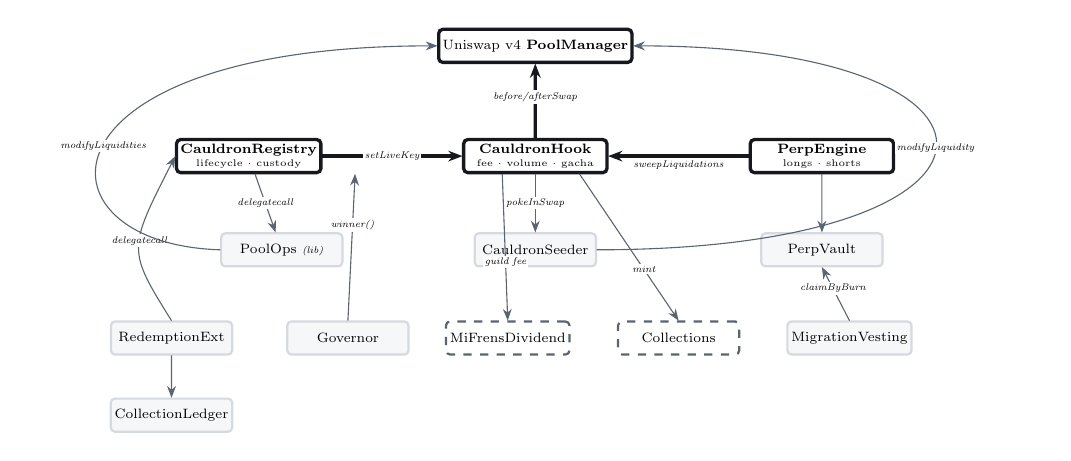
\begin{tikzpicture}[
  scale=0.70, transform shape,
  font=\scriptsize, x=1cm, y=1cm,
  box/.style={draw=rule,fill=panel,rounded corners=1.5pt,minimum height=6mm,
              minimum width=22mm,align=center,inner sep=2pt,thick},
  core/.style={box,fill=white,draw=ink,very thick,minimum width=26mm},
  ext/.style={box,fill=white,draw=slate,dashed},
  f/.style={-{Stealth[length=1.5mm]},draw=slate,thin},
  fb/.style={-{Stealth[length=1.8mm]},draw=ink,very thick},
  lbl/.style={font=\tiny\itshape,fill=white,inner sep=1pt},
]
% --- row 0: the pool -------------------------------------------------------
\node[core] (pm) at (0,4.6) {Uniswap v4 \textbf{PoolManager}};

% --- row 1: the three re-entrant cores -------------------------------------
\node[core] (reg)  at (-5.2,2.6) {\textbf{CauldronRegistry}\\[-1pt]\tiny lifecycle $\cdot$ custody};
\node[core] (hook) at ( 0.0,2.6) {\textbf{CauldronHook}\\[-1pt]\tiny fee $\cdot$ volume $\cdot$ gacha};
\node[core] (perp) at ( 5.2,2.6) {\textbf{PerpEngine}\\[-1pt]\tiny longs $\cdot$ shorts};

% --- row 2: direct collaborators -------------------------------------------
\node[box] (ops)    at (-4.6,0.9) {PoolOps \tiny\emph{(lib)}};
\node[box] (seeder) at ( 0.0,0.9) {CauldronSeeder};
\node[box] (pvault) at ( 5.2,0.9) {PerpVault};

% --- row 3: leaves ---------------------------------------------------------
\node[box] (ext)    at (-6.6,-0.7) {RedemptionExt};
\node[box] (gov)    at (-3.4,-0.7) {Governor};
\node[ext] (div)    at (-0.5,-0.7) {MiFrensDividend};
\node[ext] (col)    at ( 2.6,-0.7) {Collections};
\node[box] (vest)   at ( 5.7,-0.7) {MigrationVesting};
\node[box] (ledger) at (-6.6,-2.1) {CollectionLedger};

% --- bold: the re-entrant spine -------------------------------------------
\draw[fb] (hook) -- node[lbl,pos=0.55]{before/afterSwap} (pm);
\draw[fb] (reg.east)  -- node[lbl]{setLiveKey} (hook.west);
\draw[fb] (perp.west) -- node[lbl,below=1pt]{sweepLiquidations} (hook.east);

% --- thin: everything else -------------------------------------------------
\draw[f] (reg)  -- node[lbl,pos=0.5]{delegatecall} (ops);
\draw[f] (hook) -- node[lbl,pos=0.5]{pokeInSwap} (seeder);
\draw[f] (perp) -- (pvault);
\draw[f] (ext.north) .. controls (-7.4,0.9) .. node[lbl,pos=0.55]{delegatecall} (reg.west);
\draw[f] (gov.north) -- node[lbl,pos=0.65]{winner()} ([xshift=6mm]reg.south east);
\draw[f] (ext) -- (ledger);
\draw[f] ([xshift=-6mm]hook.south) -- node[lbl,pos=0.6]{guild fee} (div.north);
\draw[f] ([xshift=8mm]hook.south) -- node[lbl,pos=0.65]{mint} (col.north);
\draw[f] (vest.north) -- node[lbl,pos=0.6]{claimByBurn} (pvault.south);

% --- both liquidity writers reach the pool directly, routed well outside ---
\draw[f] (ops.west) .. controls (-9.2,1.0) and (-9.2,4.6) ..
      node[lbl,pos=0.5]{modifyLiquidities} (pm.west);
\draw[f] (seeder.east) .. controls (9.2,0.9) and (9.2,4.6) ..
      node[lbl,pos=0.5]{modifyLiquidity} (pm.east);
\end{tikzpicture}
\end{center}

\noindent\textbf{Reading the graph.} Bold edges are the re-entrant ones and are
where the interesting risk lives. A single user swap can, within one
\code{PoolManager} unlock, reach: the hook's \code{afterSwap} $\rightarrow$ a
nested legacy-buyback swap $\rightarrow$ the seeder's core
\code{modifyLiquidity} $\rightarrow$ the perp engine's in-lock liquidation
settlement swaps $\rightarrow$ an NFT mint. Five contracts mutating state and
settling v4 deltas inside one lock. Section~\ref{sec:failed} records why that
composition is nevertheless delta-safe.

\subsection{The two ledgers}

The single most load-bearing structural decision in the protocol is the
separation of \textbf{ledger~A} (the tradeable active band) from \textbf{ledger~B}
(the out-of-range reserve).

\begin{center}
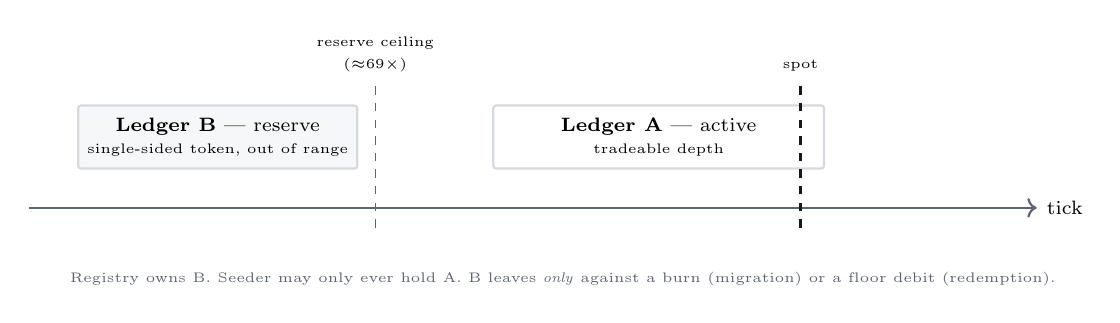
\begin{tikzpicture}[font=\scriptsize,
  band/.style={draw=rule,rounded corners=1pt,minimum height=8mm,align=center,thick}]
\draw[->,draw=slate,thick] (-0.4,0) -- (12.4,0) node[right,black]{tick};
\node[band,fill=panel,minimum width=3.4cm] (res) at (2.0,0.9) {\textbf{Ledger B} --- reserve\\\tiny single-sided token, out of range};
\node[band,fill=white,minimum width=4.2cm] (act) at (7.6,0.9) {\textbf{Ledger A} --- active\\\tiny tradeable depth};
\draw[dashed,draw=slate] (4.0,-0.25) -- (4.0,1.6) node[above,align=center]{\tiny reserve ceiling\\\tiny ($\approx$69$\times$)};
\draw[dashed,draw=ink,thick] (9.4,-0.25) -- (9.4,1.6) node[above]{\tiny spot};
\node[align=left,anchor=west] at (0.0,-0.9) {\tiny\color{slate}
Registry owns B. Seeder may only ever hold A. B leaves \emph{only} against a burn (migration) or a floor debit (redemption).};
\end{tikzpicture}
\end{center}

Everything that could drain the protocol reduces to one question: \emph{can
anything move value out of ledger~B other than a 1:1 burn or a properly-debited
floor claim?} Invariants R1--R4 in Section~\ref{sec:invariants} answer it.

\newpage
%==============================================================================
\section{Invariant register}
\label{sec:invariants}

Each invariant is stated, then argued from cited code, then given a verdict.
``Holds structurally'' means the code cannot express the violation, which is
stronger than ``holds because the arithmetic is careful.''

%------------------------------------------------------------------------------
\subsection*{S1 --- Supply is fixed and never inflates}
\textbf{Statement.} A generation's ERC-20 supply is minted once and can only ever
decrease.

\textbf{Argument.} \fileref{CauldronToken.sol:36--47}: the entire supply is minted
in the constructor to the registry. There is no \code{mint} function, no owner,
and no role that can add supply. The only supply-changing entry is
\code{burn(address,uint256)} (\fileref{:58}), gated \code{onlyRegistry}. The
contract inherits plain OpenZeppelin \code{ERC20} with no hooks that could mint.

\textbf{Verdict.} \textcolor{good}{\textbf{Holds structurally.}} The violation is
not expressible.

%------------------------------------------------------------------------------
\subsection*{S2 --- Migration is exactly 1:1 and non-duplicable}
\textbf{Statement.} Migrating $n$ old-generation tokens destroys exactly $n$ and
releases exactly $n$ of the live token; the same tokens cannot migrate twice.

\textbf{Argument.} \fileref{PoolOps.sol:656--666} (\code{migrateOne}) burns
\code{amount} from the holder and then pulls the same amount from the reserve. The
burn is real supply destruction, so the migration right cannot be replayed --- it
simply follows whoever holds the old token. The critical detail is line 665:
\begin{lstlisting}
if (got + CLAIM_DUST < amount) revert("reserve short");
\end{lstlisting}
Without it, \code{claimFromReserve} caps at the position's liquidity and returns
\emph{short without reverting}, which would let a holder burn in full and receive
less. \code{CLAIM\_DUST} is $10^{12}$ wei, covering only Uniswap's
round-down in liquidity units.

\textbf{Verdict.} \textcolor{good}{\textbf{Holds}}, with a bounded dust tolerance
of $10^{-6}$ token per claim. See F-15 for the accumulation argument.

%------------------------------------------------------------------------------
\subsection*{R1 --- The relaunch reserve covers every claimant exactly}
\textbf{Statement.} At each rebirth the new reserve is at least (old circulating
supply) + (unclaimed genesis floor) + (total legacy entitlement).

\textbf{Argument.} This is the one worth doing algebraically. Write
$T$ for \code{TOTAL\_SUPPLY}, $L$ for \code{tokensFromLP}, $G$ for
\code{genesisReserveOutstanding}, $E$ for \code{collectionLedger.totalEntitled()}.

\fileref{CauldronRegistry.sol:664--672} recovers $L$ from the dead positions and
burns it, so the old generation's remaining supply --- exactly the migration
demand --- is $T - L$. Then at \fileref{:760--790}:
\[
  A = L - G - E, \qquad R = T - A = (T - L) + G + E.
\]
The reserve is therefore \emph{exactly} the sum of the three claims, not an
approximation. Order matters and is correct: \code{\_flushLegacyAtRelaunch} and
\code{crystallizeCollection} both run \emph{before} $E$ is read at
\fileref{:774}, so late-arriving entitlements are covered.

\textbf{Verdict.} \textcolor{good}{\textbf{Holds exactly}} on the main path, as
an accounting identity. Note carefully that this is a statement about the reserve's
\emph{size}, not about its \emph{deliverability} --- see \textbf{F-18}, where the
same reserve stops being withdrawable as token despite being correctly sized.
\textcolor{medium}{Two degenerate fallbacks break even the sizing} --- one at \fileref{:763}
($L = 0$) and one at \fileref{:789} ($E \geq A$) --- both of which hard-set
$A$ to 80\% of supply and under-collateralise the reserve. See \textbf{F-06}.

%------------------------------------------------------------------------------
\subsection*{R2 --- The genesis floor only rises, or pays out its backing}
\textbf{Statement.} \code{floorPerFren()} is monotonically non-decreasing across a
recycle/resale cycle, and every payout is backed by a real reserve withdrawal.

\textbf{Argument.} \code{floorPerFren() = genesisReserveOutstanding / genesisShares}
(\fileref{CauldronBase.sol:301--305}). A recycle debits $F$ and withdraws $F$
(\fileref{RedemptionExt.sol:67--80}); the matching resale credits $2F$ and
deposits $2F$ (\fileref{:97--101}). Net $+F$ per cycle with the share count
constant, so the floor strictly ratchets. Both directions revert rather than
settle short: the redeem at \fileref{:80}, and the deposit now at \fileref{:150}
after \textbf{F-07}.

\textbf{Verdict.} \textcolor{good}{\textbf{Holds}} (F-07 closed the one path where
a payment was collected without the matching deposit landing).

%------------------------------------------------------------------------------
\subsection*{R3 --- A legacy credit never out-runs its reserve backing}
\textbf{Statement.} \code{CollectionLedger.totalEntitled} never exceeds tokens
actually deposited into the reserve or covered by the reserve's sizing.

\textbf{Argument.} The design is deliberate and good. The hook cannot deposit into
the reserve inline --- it runs nested inside \code{afterSwap} with the
\code{PoolManager} locked --- so \code{legacyBuyStep} \emph{holds} the bought
tokens and records \code{legacyOwedToReserve} (\fileref{CauldronHook.sol:831}). The
credit is only issued by \code{materializeLegacyReserve}, which deposits and
credits in one step (\fileref{RedemptionExt.sol:123--136}), crediting exactly the
swept amount. At relaunch the unmaterialised remainder is credited as a pure
number and covered by R1's sizing.

\textbf{Verdict.} \textcolor{good}{\textbf{Holds}} --- but it depended on the swept
amount being reported honestly, which \textbf{F-03} broke in the other direction
(value forgotten rather than over-credited). Now fixed and covered by invariant
\code{L-1} in the new test suite.

%------------------------------------------------------------------------------
\subsection*{R4 --- The seeder can only ever touch ledger A}
\textbf{Statement.} The progressive seeder can never reach the redemption reserve.

\textbf{Argument.} Structural. The reserve is minted by the registry through the
periphery \code{PositionManager} and the position NFT is owned by the registry
(\fileref{PoolOps.sol:479--518}). The seeder places \emph{core}
\code{poolManager.modifyLiquidity} positions owned by \emph{itself} at salt 0
(\fileref{CauldronSeeder.sol:271--281}), and its teardown iterates only its own
tracked \code{ranges} (\fileref{:291--299}). There is no code path by which the
seeder names the registry's position id.

\textbf{Verdict.} \textcolor{good}{\textbf{Holds structurally.}}

%------------------------------------------------------------------------------
\subsection*{P1 --- PLV principal sits behind collateral and insurance}
\textbf{Statement.} Depositor principal is only reduced after a position's own
collateral and the insurance buffer are exhausted.

\textbf{Argument.} Both bad-debt paths route through the buffer first:
\code{\_replenishPlv} (\fileref{PerpEngine.sol:1103--1107}) for longs and
\code{\_absorbPlvLoss} (\fileref{:1112--1118}) for shorts, each taking
\code{min(loss, insuranceEth)} before touching \code{plv}, and \code{\_absorbPlvLoss}
saturating at zero so an extreme gap cannot underflow. \code{skimInsurance}
(\fileref{:1331--1338}) protects the greater of the configured floor and a
risk-scaled minimum, so the buffer cannot be emptied while positions depend on it.

\textbf{Verdict.} \textcolor{good}{\textbf{Holds}} for the loss paths.
\textcolor{medium}{Does \emph{not} hold for funding} --- see P2.

%------------------------------------------------------------------------------
\subsection*{P2 --- Funding is a zero-sum transfer}
\textbf{Statement.} What the crowded side pays equals what the underweight side
receives.

\textbf{Argument.} It does not. \fileref{PerpEngine.sol:901--914}: the paying side
is capped by its own \code{residual} (\code{if (pay > residual) pay = residual}),
and for \emph{every} liquidated long \code{residual} is zero because
\code{repay = proceeds} leaves nothing. The receiving side draws its full claim,
capped only at \code{maxFundingBps} (50\%) of collateral, from insurance and then
from \code{plv}. The asymmetry is a net PLV outflow.

The code acknowledges this in its own comment and mitigates it by draining
insurance first. That is a real mitigation, not a fix. The remaining exposure is
bounded by the funding rate and by \code{maxFundingBps}, which is why the
unbounded \code{fundingRateBpsPerDay} (\textbf{F-04}) mattered so much: it was the
one knob that could turn a slow, bounded leak into an unbounded one.

\textbf{Verdict.} \textcolor{medium}{\textbf{Does not hold; bounded by design.}}
Documented, with the bound now enforced. See F-04 and F-16.

%------------------------------------------------------------------------------
\subsection*{V1 --- Registry and facet storage layouts are byte-identical}
\textbf{Statement.} \code{CauldronRegistry} and \code{RedemptionExt} agree
slot-for-slot, as the delegatecall pair requires.

\textbf{Argument.} Verified mechanically, not assumed. Both derive from
\code{CauldronBase} and declare no additional state. Comparing the compiled
\code{storageLayout} of both artifacts yields \textbf{53 entries, identical in
label, slot, offset and type} (reproduced in Appendix~\ref{sec:layout}). The
three former immutables (\code{poolManager}, \code{positionManager}, \code{hook})
are correctly \emph{storage} at slots 41--43; as immutables they would resolve to
zero inside the facet, since immutables live in the executing contract's own code.

One subtlety worth recording: OpenZeppelin 5.6's \code{ReentrancyGuard} uses an
ERC-7201 \emph{namespaced} slot, not a sequential one, so it appears in neither
layout and is shared correctly under delegatecall. That is why the registry's
forwarders must \emph{not} carry \code{nonReentrant} --- they would double-lock
against the facet's own guard. \fileref{CauldronRegistry.sol:1081--1084} states
this and \fileref{:1089--1109} implements it correctly.

\textbf{Verdict.} \textcolor{good}{\textbf{Holds, mechanically verified.}}
See \textbf{F-13} for a tooling gap in the documented verification procedure.

%------------------------------------------------------------------------------
\subsection*{V2 --- Every v4 delta is settled}
\textbf{Statement.} No path leaves a \code{PoolManager} delta unsettled or
double-settled.

\textbf{Argument.} Four contracts settle inside a single unlock. Each was checked:
\begin{itemize}
\item \code{PoolOps.executeBuy} (\fileref{:361--388}) settles \code{ethIn} and takes
\code{got}, both read from the returned delta rather than from the intent.
\item \code{CauldronHook.legacyBuyStep} (\fileref{:800--833}) settles the
\emph{realised} debit \code{-d.amount0()}, not the intended \code{amt}, and returns
the unspent remainder to the buffer. Settling the intent would leave a positive
un-taken delta and revert the user's parent swap.
\item \code{PerpEngine.\_swapBody} (\fileref{:968--992}) settles and takes both legs,
and correctly runs \emph{in place} when \code{\_inLocked} rather than re-entering
\code{unlock}, which would revert.
\item \code{CauldronSeeder.\_settle} (\fileref{:343--358}) nets both
\code{modifyLiquidity} deltas and settles the aggregate, handling each currency in
either direction, with \code{sync} before the ERC-20 settle.
\end{itemize}
The hook's fee take is the standard v4 pattern: \code{poolManager.take} of exactly
\code{total}, offset by returning the same \code{total} as the hook delta on the
unspecified currency (\fileref{CauldronHook.sol:1103}, \fileref{:750}).

\textbf{Verdict.} \textcolor{good}{\textbf{Holds}} on all four paths.

%------------------------------------------------------------------------------
\subsection*{L1 --- The death clock is denominated in wall-clock time}
\textbf{Statement.} Pool retirement depends on elapsed seconds, not block count.

\textbf{Argument.} \fileref{CauldronHook.sol:136--138, 1134--1192}: the window uses
\code{SECONDS\_PER\_HOUR} / \code{SECONDS\_PER\_DAY} against \code{\_lastUpdateTs},
a \code{block.timestamp}. This is the correct choice for the target and the
report verifies it by simulation: \code{test\_L2A\_DeathClockIsWallClockNotBlockCount}
advances 50{,}000 blocks with time frozen (nothing dies) and then a day of
wall-clock with only parent-chain-sized block motion (it dies on schedule).

\textbf{Verdict.} \textcolor{good}{\textbf{Holds; L2-correct.}}

%------------------------------------------------------------------------------
\subsection*{L2 --- Per-block guards remain per-block on the target}
\textbf{Statement.} Guards that must bound activity per block still do so when
\code{block.number} is the parent chain's.

\textbf{Argument.} Split verdict.
\begin{itemize}
\item The perp liquidation throttle is keyed on \code{block.timestamp}
(\fileref{PerpEngine.sol:206, 637, 726}) --- \textbf{correct}, and the code says
exactly why. On Orbit a \code{block.number} key would let one cap span dozens of
child blocks.
\item The anti-snipe surtax is keyed on \code{block.number}
(\fileref{CauldronHook.sol:1046}) --- \textbf{quantised}. It keeps its intended
\emph{wall-clock} length but loses per-block resolution. See \textbf{F-11}.
\end{itemize}

\textbf{Verdict.} \textcolor{medium}{\textbf{Partially holds.}}

\newpage
%==============================================================================
\section{Findings}
\label{sec:findings}

\begin{longtable}{@{}llp{0.44\linewidth}ll@{}}
\toprule
\textbf{ID} & \textbf{Sev} & \textbf{Title} & \textbf{Conf.} & \textbf{Status} \\
\midrule\endhead
F-18 & \SevHigh & Success voids the exit guarantee at the reserve ceiling & \Conf & Documented \\
F-01 & \SevHigh & Protocol randomness relies on \code{blockhash}, documented unsafe on the target chain & \Susp & Documented \\
F-02 & \SevMed & Auto-migrate consent is irrevocable & \Conf & \textcolor{good}{Fixed} \\
F-03 & \SevMed & Legacy sweep silently forgets owed value & \Conf & \textcolor{good}{Fixed} \\
F-04 & \SevMed & Unbounded funding rate inverts or bricks the perp engine & \Conf & \textcolor{good}{Fixed} \\
F-05 & \SevMed & Seeder range-cap fallback can mis-side a band and halt the stream & \Conf & \textcolor{good}{Fixed} \\
F-09 & \SevMed & Dividend hook is gas-starvable: fee bypass and value transfer & \Conf & \textcolor{good}{Fixed} \\
F-11 & \SevMed & Anti-snipe surtax is quantised to parent blocks & \Conf & Documented \\
F-12 & \SevMed & \code{MIN\_TWAP} of 1\,s is not a meaningful floor on a fast L2 & \Conf & Documented \\
F-19 & \SevMed & A zero \code{emergencyDelay} silently voids the forced-open exit & \Conf & \textcolor{good}{Fixed} \\
F-06 & \SevLow & Silent under-collateralised reserve fallback & \Conf & \textcolor{good}{Fixed} \\
F-07 & \SevLow & Payment collected when the reserve deposit cannot land & \Conf & \textcolor{good}{Fixed} \\
F-08 & \SevLow & One short holder reverts the whole auto-migrate batch & \Conf & \textcolor{good}{Fixed} \\
F-10 & \SevLow & \code{uint32} epoch rollover panics the TWAP oracle & \Conf & \textcolor{good}{Fixed} \\
F-14 & \SevLow & EIP-170 headroom is nearly exhausted & \Conf & Documented \\
F-16 & \SevLow & \code{enableAutoMigrate} keeps overpayment & \Conf & Documented \\
F-13 & \SevInfo & Documented layout-verification command does not run & \Conf & Documented \\
F-15 & \SevInfo & Funding overflow at an extreme mark & \Susp & Documented \\
F-17 & \SevInfo & \code{CauldronVault.redeem} is permanently unreachable as configured & \Conf & Documented \\
\bottomrule
\end{longtable}

\newpage
\subsection{F-01 --- Protocol randomness relies on \texorpdfstring{\code{blockhash}}{blockhash}}

\begin{findingbox}{high}{F-01 \quad \textbf{High}\quad Confidence: Suspected (chain-dependent) \quad Status: documented}
\textbf{Location.} \fileref{CauldronHook.sol:1732, 1754} (crystal gacha);
\fileref{CauldronCollection.sol:215, 232} and \fileref{MiFrensGenesis.sol:417, 434}
(rarity reveal); \fileref{CauldronHook.sol:1064} (surtax jitter).
\end{findingbox}

\subsubsection*{What the code does}

Three independent mechanisms derive an outcome from \code{blockhash}. The gacha is
the economically significant one:

\begin{lstlisting}
// CauldronHook._resolveTickets, lines 1731-1754
if (block.number <= b.commitBlock) break;          // maturity gate
bytes32 bh = blockhash(b.commitBlock);
...
uint256 roll = uint256(keccak256(abi.encodePacked(bh, player, bi, r))) % 10_000;
bool win = (forced || roll < odds) && minted < max;
if (win) { ... ICauldronCollection(col).mint(player); }
\end{lstlisting}

The design is a proper commit--reveal: \code{oddsBps} is fixed at commit,
\code{commitBlock} is the current block, and the seed is a value that does not
exist yet. On Ethereum that is sound.

\subsubsection*{Why the target chain changes the conclusion}

Arbitrum's own documentation is explicit on all three points that matter:

\begin{itemize}
\item \code{blockhash(x)} ``[r]eturns a cryptographically insecure, pseudo-random
hash for \code{x} within the range \code{block.number - 256 <= x < block.number}'';
\item ``The hashes returned do not come from L1'';
\item ``Arbitrum's child chain block hashes should not be relied on as a secure
source of randomness'', with Chainlink VRF given as the recommended alternative.
\end{itemize}

\noindent The Robinhood Chain documentation repeats this: ``\code{blockhash(n)} is
supported but is only reliable for recent blocks'', and warns against using it as
a randomness source.

Compounding it, \code{block.number} on the target ``returns an estimate of the L1
(Ethereum) block number \dots and updates only periodically.'' So the maturity
gate \code{block.number > commitBlock} is satisfied roughly once per parent block,
and every child block inside that window shares one \code{commitBlock} value ---
which means one seed governs every crystal committed across dozens of child
blocks.

\subsubsection*{Impact}

If the pseudo-random derivation is predictable --- which is what
``cryptographically insecure'' warns of --- then the roll is fully determined at
commit time, because it is a pure function of four values a player either
controls or can compute. A player can then commit only when the outcome is a win.
The same argument applies to \code{reveal()}, where the payoff is a rarity tier
with direct secondary-market value.

Even without predictability, the single sequencer's first-come-first-served
ordering gives whoever operates it discretion over which transactions land in
which block, and therefore over which seed each commit is anchored to.

\subsubsection*{Evidence}

\code{test\_L2C\_RollIsFullyDeterminedByBlockhash} in
\fileref{test/final/F02\_L2Semantics.t.sol} makes the dependency machine-checked:
it commits a batch, matures it, reads \code{blockhash(commitBlock)}, and shows
that recomputing $\mathrm{keccak}(bh,\,player,\,bi,\,r) \bmod 10^4$ off-chain
reproduces the contract's roll exactly. It asserts a property, not an exploit:
\emph{the outcome carries no entropy beyond the blockhash.}

\subsubsection*{Why no code fix is shipped here}

\code{CauldronHook} has \textbf{88 bytes} of EIP-170 headroom
(24{,}488 / 24{,}576). Every structural remedy --- an entropy accumulator fed by
each swap, a pluggable \code{IEntropy} module, a two-phase reveal --- costs
several hundred bytes. Shipping a half-measure that fits would be worse than
documenting the real one.

\subsubsection*{Remediation, in priority order}

\begin{enumerate}
\item \textbf{Verify the derivation on the target before launch.} Deploy a
one-function probe that records \code{blockhash(block.number - 1)} over a few
hundred blocks and check whether the sequence is a function of the block number
alone. This is a half-hour task and it decides everything below. Until it is
done, treat the gacha odds as advisory.
\item \textbf{If predictable: make the seed a third party's future action.}
Reclaim bytes first (F-14 lists candidates --- \code{CauldronVault} integration is
vestigial per F-17), then add a hook-level entropy accumulator updated on every
swap and require a batch's resolve to consume an accumulator value written
\emph{after} its commit. The seed then depends on other traders' behaviour, which
the committer cannot predict or produce alone.
\item \textbf{Alternative: wire Chainlink VRF} if available on the target, via a
policy module rather than in the hook, so the hook's size is unaffected.
\item \textbf{Interim mitigation, zero bytes:} widen the maturity gap. Requiring
several parent blocks between commit and resolve does not fix predictability, but
it removes same-block commit-and-resolve and raises the cost of any ordering game.
\end{enumerate}

\subsubsection*{Not affected: \texorpdfstring{\code{prevrandao}}{prevrandao}}

Worth stating explicitly, because it is the more common version of this bug.
Arbitrum returns \textbf{the constant 1} for both \code{block.prevrandao} and
\code{block.difficulty}. A grep of the entire in-scope corpus finds \textbf{zero}
uses of either. \fileref{CauldronHook.sol:1055--1061} documents that this was a
deliberate migration away from \code{prevrandao}. That is correct, and it is the
right instinct applied one step short of the conclusion --- the replacement
(\code{blockhash} plus the live tick) inherits the same class of weakness.

\newpage
\subsection{F-18 --- Success voids the exit guarantee at the reserve ceiling}

\begin{findingbox}{high}{F-18 \quad \textbf{High}\quad Confidence: Confirmed (reproduced on a live pool) \quad Status: documented}
\textbf{Location.} \fileref{ReserveLib.sol:50--66} (\code{reserveTicks}),
\fileref{PoolOps.sol:555--584} (\code{claimFromReserve}), \fileref{:665}
(\code{migrateOne}'s short guard), \fileref{RedemptionExt.sol:80},
\fileref{CauldronRegistry.sol:180--182} (\code{setReserveCeiling}),
\fileref{:1428--1434} (\code{floorClaimableNow}).
\end{findingbox}

\subsubsection*{The mechanism}

The migration reserve is a single-sided \emph{token} position parked out of range.
Its band is placed \code{RESERVE\_CEILING\_OFFSET} ticks below the launch tick ---
42{,}400 by default, about $69\times$ --- and \code{ReserveLib} is explicit about the
orientation:

\begin{quote}\small\itshape
``the reserve must sit BELOW the launch tick: it is pure token while
\code{currentTick > reserveTickUpper}, and only begins converting to ETH if the
token pumps ${\sim}69\times$ down into the range.''
\end{quote}

That parenthetical is the finding. Everything downstream assumes the band delivers
\emph{pure token1}: \code{claimFromReserve} sizes a withdrawal with
\code{liquidityForTokenOut}, which is only the inverse of the position's contents
while the range is entirely below spot. Once the token appreciates through the
ceiling, the band is \emph{in range}: removing that liquidity yields a mix of ETH
and token, so the token delivered falls short of the amount asked for --- and every
consumer that demands the full amount reverts:

\begin{itemize}
\item \code{migrateOne} reverts \code{"reserve short"} (\fileref{PoolOps.sol:665}),
closing 1:1 migration for \emph{every} holder of \emph{every} prior generation;
\item \code{redeemOgFren} reverts \code{NoBalance} (\fileref{RedemptionExt.sol:80}),
closing the OG floor;
\item \code{recycleCollectionNFT} reverts on the same guard
(\fileref{PoolOps.sol:780}), closing every collection floor.
\end{itemize}

Those reverts are individually \emph{correct} --- each exists so a holder never
burns in full and receives less. The problem is what they compose into.

\subsubsection*{Why this is High rather than a design note}

Three things make it serious.

\textbf{It fires on success, not on failure.} Every other risk in this protocol is
triggered by something going wrong. This one triggers when the token does exactly
what everyone wants. The exit guarantee is advertised without qualification --- the
registry describes the reserve as what ``backs migration/genesis 1:1'' --- and it
silently stops holding at precisely the moment holders most want to use it.

\textbf{It cannot be repaired for the live generation.}
\code{setReserveCeiling} is explicit that it applies to ``the NEXT summon/relaunch''
(\fileref{CauldronRegistry.sol:176--182}); the live band's ticks were fixed at
seed time and are stored per-generation in \code{reserveTickUpper[gen]}. The only
way to re-place a reserve is a relaunch --- which requires \code{hook.isDead()},
i.e.\ 24-hour volume below the threshold. A token that just appreciated
$69\times$ is the least likely thing on the chain to be quiet. The system is
therefore self-locking: the condition that breaks the exit is also the condition
that prevents the repair.

\textbf{The break is total, not proportional.} It is not that holders receive less;
it is that the transaction reverts entirely. There is no partial exit, no
degraded-but-working path.

\subsubsection*{Reproduction}

\code{test\_F18\_MigrationBreaksAboveTheCeiling}
(\fileref{test/final/F04\_ReserveCeiling.t.sol}) drives it on live Uniswap v4:
summon with a genesis bonus, acquire circulating supply while migration works, then
buy repeatedly until \code{slot0.tick} falls to or below
\code{reserveTickUpper(1)}. At that point it asserts, in order:

\begin{enumerate}
\item \code{registry.floorClaimableNow()} returns \code{claimable == false};
\item \code{claimByBurn(1, circulating)} reverts;
\item \code{redeemOgFren(1)} reverts;
\item the holder's balance and their fren are both untouched.
\end{enumerate}

The companion \code{test\_F18\_MigrationWorksBelowTheCeiling} shows both paths
succeeding at the same configuration before the pump, so the difference is the
price and nothing else. \code{test\_F18\_CeilingIsSetBeforeTheSummonOnly} confirms
that calling \code{setReserveCeiling(138000)} afterwards leaves
\code{reserveTickUpper(1)} unchanged.

\subsubsection*{What the protocol already does about it}

Worth crediting: \code{floorClaimableNow} (\fileref{CauldronRegistry.sol:1428})
exists precisely to surface this state --- it returns
\code{claimable = tick > reserveTickUpper[g]}. So the condition is known and is
exposed to the frontend. What is missing is any \emph{on-chain} remedy: the view
tells a holder their exit is closed, but nothing lets them or governance reopen it.

\subsubsection*{Remediation}

No code fix is applied here because every option is a design decision with real
economic consequences, and this is the kind of change that should be chosen by the
protocol's authors rather than by its auditor. In rough order of cost:

\begin{enumerate}
\item \textbf{Set the ceiling deliberately, per iteration.} The setter's bounds
(4{,}000 to 138{,}000 ticks, roughly $1.5\times$ to $10^6\times$) are wide enough
that a launch expecting more than $69\times$ can simply say so \emph{before} the
summon. This is free, it is already possible today, and it should be an explicit
line item in the launch runbook rather than a default nobody revisits. It narrows
the window; it does not close it.

\item \textbf{Add a governance-gated reserve \emph{re-placement}} --- withdraw the
reserve position and re-mint it at a band below the new spot, without touching the
active book. This is the real fix. It is a custody action, so it belongs behind the
existing \code{armEmergency} / \code{timelocked} / guardian-veto machinery, and
under the exit-guarantee rule already in \code{\_redeemBlocked} the redemption path
is forced open while it is armed. Registry headroom is 339 bytes, so this likely
needs a \code{PoolOps} entry plus a thin forwarder.

\item \textbf{Alternatively, make the short path graceful.} Let
\code{claimFromReserve} deliver token \emph{and} the ETH the band converted into,
valuing the pair at the mark, so a holder exits at fair value rather than not at
all. This changes the meaning of ``1:1'' and would need to be stated plainly to
holders --- which is why it ranks below (2).
\end{enumerate}

\noindent Until one of these lands, the honest statement of the guarantee is:
\emph{migration and the redemption floor are available while the token trades below
its per-iteration reserve ceiling.} That qualification should appear anywhere the
guarantee is described.

\newpage
\subsection{F-02 --- Auto-migrate consent is irrevocable}

\begin{findingbox}{medium}{F-02 \quad \textbf{Medium}\quad Confidence: Confirmed \quad Status: \textbf{Fixed}}
\textbf{Location.} \fileref{CauldronRegistry.sol:1027--1037} (\code{enableAutoMigrate}),
\fileref{:1046--1062} (\code{autoMigrateBatch}), \fileref{CauldronBase.sol:259}.
\end{findingbox}

\subsubsection*{The defect}

\code{enableAutoMigrate} sets \code{autoMigrate[msg.sender] = true}. No function
anywhere in the corpus sets it back to \code{false} --- verified by grep across
\code{CauldronRegistry.sol}, \code{CauldronBase.sol} and \code{PoolOps.sol}: the
only writes are that one line and the reads in
\fileref{PoolOps.sol:677}.

That flag is the sole gate on \code{autoMigrateBatch}, which calls
\code{migrateOne} $\rightarrow$ \code{ICauldronBurn(prevToken).burn(h, bal)}. Note
what that primitive is: \code{CauldronToken.burn} is \code{onlyRegistry} and takes
an arbitrary \code{from} (\fileref{CauldronToken.sol:58--60}). It needs no
allowance. So an opted-in wallet has handed any permissionless keeper standing
authority to destroy its entire old-generation balance, at any future relaunch, at
a moment of the keeper's choosing.

\subsubsection*{Why this matters more than it first appears}

The registry's own documentation of \code{claimByBurn} states the model plainly
(\fileref{:931--935}): ``\emph{OPTIONALLY migrate \dots Migration is a choice, not
a requirement --- old tokens are never frozen, so a holder who prefers a past
iteration simply keeps (or trades) it.}''

A holder who paid 0.069~ETH for convenience during iteration~3 and then decided
they prefer iteration~7 had no way to stop the machine converting them. Their
only escape was to move their balance to a fresh address --- which is not a
remedy, it is a workaround for a missing function. The consent is also
\emph{unpriced in time}: it was granted under one set of conditions and is
exercised under another, possibly years later.

\subsubsection*{Fix applied}

\begin{lstlisting}
/// @notice Revoke the hands-off migration consent (audit F-02).
function disableAutoMigrate() external {
    autoMigrate[msg.sender] = false;
    emit AutoMigrateSet(msg.sender);
}
\end{lstlisting}
Free --- revoking a permission must never sit behind a fee --- and effective
immediately, because \code{PoolOps.autoMigrateBatch} reads the flag per holder per
call. Re-opting in costs the fee again, so this is not a fee bypass.

\subsubsection*{Tests}

\code{test\_F02\_AutoMigrateConsentIsRevocable} and
\code{test\_F02\_RevocationIsSelfServiceOnly}
(\fileref{test/final/F01\_CustodyAndConsent.t.sol}), plus the handler-driven
invariant \code{invariant\_C1\_ConsentMatchesTheActorsLastChoice}
(\fileref{test/final/F03\_FinalInvariants.t.sol}), which fuzzes opt-in/opt-out
sequences across three actors and asserts the on-chain flag always equals that
actor's own last instruction --- 128{,}000 calls, no violation.

\newpage
\subsection{F-03 --- Legacy sweep silently forgets owed value}

\begin{findingbox}{medium}{F-03 \quad \textbf{Medium}\quad Confidence: Confirmed \quad Status: \textbf{Fixed}}
\textbf{Location.} \fileref{CauldronHook.sol:848--855} (\code{sweepLegacyReserve}).
\end{findingbox}

\subsubsection*{The defect}

\begin{lstlisting}
amt = legacyOwedToReserve;
legacyOwedToReserve = 0;                                  // <-- unconditional
uint256 bal = IERC20(token).balanceOf(address(this));
if (amt > bal) amt = bal;                                 // <-- clamp AFTER
if (amt > 0) IERC20(token).transfer(to, amt);
\end{lstlisting}

The counter is zeroed \emph{before} the transfer is clamped to the live balance.
In any state where \code{balance < owed}, the difference is destroyed: the tokens
remain in the hook, are credited to no collection's floor, and no later sweep can
find them, because the only record that they were owed has been erased. The
function is the sole consumer of that counter
(\fileref{PoolOps.sol:725}), so the loss is unrecoverable without a redeploy.

\subsubsection*{Severity reasoning}

Rated Medium rather than High because reaching \code{balance < owed} requires a
desynchronisation between the counter and the hook's token balance, and the two
are written together in \code{legacyBuyStep} (\fileref{:823--831}). It is rated
Medium rather than Low because the failure is \emph{silent and permanent}, the
function is reachable permissionlessly through
\code{materializeLegacyReserve}, and the value it guards is every NFT holder's
floor. A counter whose only job is to remember value should not be able to forget
it under any input.

\subsubsection*{Fix applied}

\begin{lstlisting}
uint256 owed = legacyOwedToReserve;
uint256 bal  = IERC20(token).balanceOf(address(this));
amt = owed > bal ? bal : owed;
legacyOwedToReserve = owed - amt;        // debit exactly what moved
if (amt > 0) IERC20(token).transfer(to, amt);
\end{lstlisting}
Invariant R3 is preserved in both directions: the registry credits exactly the
returned \code{amt}, so a credit still cannot out-run the reserve, and now the
remainder stays claimable by the next sweep.

\subsubsection*{Evidence that the test catches it}

Reverting the fix and re-running:
\begin{center}\small
\begin{tabular}{@{}lp{0.62\linewidth}@{}}
\toprule
\textbf{Test} & \textbf{Result against pre-fix bytecode} \\
\midrule
\code{test\_F03\_PartialSweep...} & \code{FAIL: remainder still owed: 0 != 60000000000000000000} \\
\code{testFuzz\_F03\_SweepDebits...} & \code{FAIL: counter debited by exactly the move: 0 != 19998686626960} \\
\code{invariant\_L1\_NoOwedValue...} & \code{FAIL: 1441207360336501672073743 != 2284619084570732192188892} \\
\bottomrule
\end{tabular}
\end{center}
The invariant is the strongest of the three: across 128{,}000 fuzzed handler calls
it showed roughly $8.4\times10^{23}$ base units silently vanishing. All three pass
against the fixed contract.

\newpage
\subsection{F-04 --- Unbounded funding rate inverts or bricks the perp engine}

\begin{findingbox}{medium}{F-04 \quad \textbf{Medium}\quad Confidence: Confirmed \quad Status: \textbf{Fixed}}
\textbf{Location.} \fileref{PerpEngine.sol:1258--1267} (\code{setRisk}),
\fileref{:504--521} (\code{\_pokeFunding}).
\end{findingbox}

\subsubsection*{The defect}

\code{setRisk} validates every parameter it takes except one:

\begin{lstlisting}
if (_warmup < MIN_TWAP) revert BadParam();
if (!(_ceiling >= 1 && _ceiling <= 10 && _maintBps <= 5000
      && _maxNotBps <= BPS && _maxOiBps <= BPS)) revert BadParam();
...
fundingRateBpsPerDay = _fundingBpsDay;      // no bound at all
\end{lstlisting}

That value is then used in signed 256-bit arithmetic:
\begin{lstlisting}
int256 step = (imbalance * int256(fundingRateBpsPerDay) * int256(dt) * 1e18)
            / (int256(total) * int256(BPS) * int256(1 days));
\end{lstlisting}

Two distinct failures follow.

\textbf{Sign inversion.} For any value at or above $2^{255}$, the
\code{int256} cast wraps negative. \code{step} flips sign, so the funding index
moves the wrong way and \emph{the crowded side gets paid} by the underweight side
--- through the PLV, via the non-conservative path documented under invariant P2.

\textbf{Permanent brick.} For a merely large value, the checked multiplication
overflows and \code{\_pokeFunding} reverts. This is the serious one, because of
what calls it: \code{openLong}, \code{openShort}, \code{close}, \code{liquidate},
\code{forceCloseDead}, \code{forceCloseAllDead}, \code{\_doSweep} and \code{poke}
--- every mutating entrypoint. A reverting \code{forceCloseAllDead} means
\code{openCount} never returns to zero, which means \code{syncGeneration} reverts
\code{PositionsOpen} forever (\fileref{:783}), which strands the entire token-side
inventory in a dead generation with no recovery path.

\subsubsection*{Reachability}

Governance only (\code{onlyOwner}, the timelock on mainnet), so this is a
fat-finger and compromised-governance concern rather than an open attack. It is
still worth Medium: it is a one-call, irreversible loss of the whole perp
subsystem, and every sibling parameter on the same setter is already bounded ---
the omission looks like an oversight rather than a decision.

\subsubsection*{Fix applied}

\begin{lstlisting}
if (!(_ceiling >= 1 && _ceiling <= 10 && _maintBps <= 5000 && _maxNotBps <= BPS
    && _maxOiBps <= BPS && _fundingBpsDay <= BPS)) revert BadParam();
\end{lstlisting}
100\% of notional per day is already far beyond any defensible funding rate, and
it caps P2's structural leak at a knowable rate.

\subsubsection*{Tests}

\code{test\_L2D\_FundingRateIsBounded} rejects $2^{255}$,
\code{type(uint256).max} and $10^4+1$, and confirms the ceiling and the shipped
default remain settable. \code{testFuzz\_L2D\_PokeSurvivesAnyAcceptedRate} then
fuzzes every accepted rate against a year of decoupled clock advance and asserts
\code{poke()} never reverts.

\newpage
\subsection{F-05 --- Seeder range-cap fallback can mis-side a band}

\begin{findingbox}{medium}{F-05 \quad \textbf{Medium}\quad Confidence: Confirmed \quad Status: \textbf{Fixed}}
\textbf{Location.} \fileref{CauldronSeeder.sol:370--381} (\code{\_reserveRange}),
\fileref{:241--283} (\code{\_placeStep}).
\end{findingbox}

\subsubsection*{The defect}

The seeder bounds teardown gas by tracking at most \code{MAX\_RANGES = 64} distinct
tick bands. At the cap it degrades rather than halting --- a deliberate and correct
choice --- but it degraded to the wrong thing:

\begin{lstlisting}
if (n >= MAX_RANGES) {
    Range storage r = ranges[n - 1];    // the most recently PUSHED range
    return (r.lo, r.hi);                // ...whichever side of spot it is on
}
\end{lstlisting}

\code{\_placeStep} reserves the \emph{ask} band and then the \emph{bid} band, so at
the cap both resolve to that same single range. The two sides are then sized with
opposite formulas (\fileref{:262--267}): \code{getLiquidityForAmount1} for the ask
(pure \code{token1}, band \emph{below} spot) and \code{getLiquidityForAmount0} for
the bid (pure \code{token0}/ETH, band \emph{above} spot).

Feeding an ask amount into a band above spot mints a position the pool settles
entirely in ETH. \code{\_settle} is then asked for an ETH debit bearing no relation
to \code{ethStep} --- and which the seeder does not hold --- so the placement
reverts. In-swap that is swallowed by the hook's gas-bounded call; via the
permissionless \code{poke()} it is a hard revert. Either way the stream halts,
which is precisely what the degrade-don't-halt design existed to prevent.

\subsubsection*{Reachability}

Real, not theoretical. A new range is tracked each time the aligned tick moves one
spacing (\fileref{:254--260} via \code{SeedLib.askBand}/\code{bidBand}). At
\code{spacing = 200}, exhausting 64 ranges takes roughly 64 spacings of tick drift
--- comfortably inside one launch window of genuine trading, which is exactly the
period the progressive seed is designed for.

\subsubsection*{Fix applied}

Track the last band \emph{per side} and fall back to the matching one, so an ask
always degrades into an ask and a bid into a bid:
\begin{lstlisting}
function _reserveRange(int24 lo, int24 hi, bool isAsk) private returns (int24, int24) {
    ...
    if (n >= MAX_RANGES) {
        Range storage r = isAsk ? _lastAsk : _lastBid;
        if (r.lo == 0 && r.hi == 0) return (0, 0);   // decline rather than mis-side
        return (r.lo, r.hi);
    }
    ...
}
\end{lstlisting}
Three supporting changes: \code{\_lastAsk}/\code{\_lastBid} are cleared in
\code{startSeed} alongside \code{ranges} (they are tick coordinates in the previous
generation's pool); the two-sided full-range \emph{base} is pushed directly rather
than through \code{\_reserveRange}, so it never becomes either side's fallback; and
\code{\_placeStep} guards \code{hi > lo} before sizing, since a declined band would
otherwise divide by zero.

\subsubsection*{Note on residual behaviour}

At the cap the stream continues into an increasingly stale band. That is the
intended degradation and nothing is stranded --- the band is tracked, so
\code{withdrawAll} still recovers it. The invariant that matters is preserved:
\emph{the seeder never places into an untracked range.}

\newpage
\subsection{F-09 --- The dividend hook is gas-starvable}

\begin{findingbox}{medium}{F-09 \quad \textbf{Medium}\quad Confidence: Confirmed (window measured) \quad Status: \textbf{Fixed}}
\textbf{Location.} \fileref{MiFrensGenesis.sol:559--561} (\code{\_update}),
\fileref{MiFrensDividend.sol:224--233} (\code{onMiFrenTransfer}),
\fileref{:191--194} (the stale branch of \code{\_castSpell}).
\end{findingbox}

\subsubsection*{The defect}

\begin{lstlisting}
if (from != address(0) && dividend != address(0)) {
    try IMiFrensDividendHook(dividend).onMiFrenTransfer(tokenId, from) {} catch {}
}
\end{lstlisting}

\code{try/catch} swallows an out-of-gas child exactly as readily as a genuine
revert, and EIP-150 forwards only $63/64$ of the remaining gas. A seller who sizes
their transaction's gas precisely can therefore make this child call run out of
gas while the transfer itself still settles.

\subsubsection*{Why the first attempt at this attack failed, and what fixed it}

This is worth recording because it changed the verdict twice.

The obvious version does \emph{not} work. For a \textbf{genesis} fren the code
after the dividend call includes an \code{everMoved} SSTORE
(\fileref{:565--567}), costing $\geq 20{,}000$ gas. If the child is starved, the
parent resumes with only $1/64$ of the gas --- a few hundred units --- and cannot
pay for that write, so the whole transfer reverts. A gas sweep from 60k to 260k in
5k steps confirmed it: at every budget where the transfer succeeded, the hook had
run.

The attack works on the \textbf{forged} tranche. That SSTORE is guarded by
\code{tokenId <= GENESIS\_SUPPLY}, so for a volume-minted fren
(\code{id > GENESIS\_SUPPLY}) the post-call work is nearly free and the $1/64$
remainder covers it. Re-running the sweep against a forged fren:

\begin{center}\small
\begin{tabular}{@{}rcl@{}}
\toprule
\textbf{Gas budget} & \textbf{Transfer settles?} & \textbf{\code{activeShares} after} \\
\midrule
$\leq$ 115{,}000 & no & --- \\
\rowcolor{panel!80} 117{,}500 -- 130{,}000 & \textbf{yes} & \textbf{1} \quad\textcolor{critical}{$\leftarrow$ hook starved} \\
$\geq$ 132{,}500 & yes & 0 \quad(hook ran) \\
\bottomrule
\end{tabular}
\end{center}

A deterministic window roughly 13{,}000 gas wide, hit at will.

\subsubsection*{Impact}

Three consequences, and they are precisely the ones the M-06 comment in that same
function says it exists to prevent --- reachable on demand:

\begin{enumerate}
\item \textbf{Permanent dilution.} \code{enchantedBy[tokenId]} still points at the
seller, so the fren stays counted in \code{activeShares} while earning for nobody.
Every honest holder's share of every future fee is reduced, indefinitely.
\item \textbf{Backwards value transfer.} When the buyer eventually re-casts, the
stale branch of \code{\_castSpell} credits
\code{owed[cur] += (accPerShare - debtOf[tokenId]) / ACC} --- paying the
\textbf{seller} for the accrual earned while the \textbf{buyer} owned the NFT.
\item \textbf{Fee bypass.} That stale branch never calls
\code{\_collectEnchantFee} (\fileref{:191--194} versus \fileref{:183--190}), so the
buyer re-enchants free, dodging the reserve-growing fee a moved fren is supposed
to pay --- and forged frens are exactly the tranche that always pays it.
\end{enumerate}

\subsubsection*{Fix applied}

\begin{lstlisting}
if (from != address(0) && dividend != address(0)) {
    if (gasleft() < GAS_DIVIDEND_MIN) revert InsufficientGas();     // 80_000
    try IMiFrensDividendHook(dividend).onMiFrenTransfer{gas: GAS_DIVIDEND_FWD}(tokenId, from) {}
    catch {}
}
\end{lstlisting}

The hook's work is a fixed, small set of storage writes --- worst case about 39k,
dominated by one cold zero-to-non-zero \code{owed} SSTORE plus three cold non-zero
updates. Requiring 80k before attempting it, and forwarding an explicit 60k,
removes the attacker's ability to \emph{choose} failure while keeping the property
that a genuinely broken dividend can never brick a transfer: a real revert is
still caught. Mints (\code{from == 0}) never reach this branch, so the in-protocol
badge and art mint paths are untouched.

\subsubsection*{Tests}

\code{test\_F09\_Gas\-Starved\-Transfer\-Is\-Refused} targets the measured
window's midpoint. \code{test\_F09\_The\-Entire\-Grief\-Window\-Is\-Closed} sweeps
110k--132k in 2k steps and asserts the property directly --- \emph{a settled transfer always breaks
the spell} --- so the fix cannot be evaded by retuning gas. Two control tests
confirm normal transfers still settle and a reverting dividend still cannot brick
one. Against the pre-fix bytecode the first two fail
(\code{FAIL: gas-starved transfer must not settle} and
\code{FAIL: a settled transfer always breaks the spell: 1 != 0}) while both
controls pass.

\newpage
\subsection{F-19 --- A zero \texorpdfstring{\code{emergencyDelay}}{emergencyDelay} silently voids the forced-open exit}

\begin{findingbox}{medium}{F-19 \quad \textbf{Medium}\quad Confidence: Confirmed (observed on the live deployment) \quad Status: \textbf{Fixed}}
\textbf{Location.} \fileref{CauldronBase.sol:311--313} (\code{\_redeemBlocked}),
\fileref{CauldronRegistry.sol:250--255} (\code{\_consumeTimelock}),
\fileref{:159} (the \code{immutable} assignment).
\end{findingbox}

\subsubsection*{The interaction}

Two guards that are individually correct compose into a silent hole:

\begin{lstlisting}
// CauldronBase -- THE EXIT GUARANTEE
function _redeemBlocked() internal view returns (bool) {
    return redemptionPaused && emergencyReadyAt == 0;
}
// CauldronRegistry -- the delay is OPTIONAL
function _consumeTimelock() private {
    if (emergencyDelay != 0) { ... emergencyReadyAt = 0; }
}
\end{lstlisting}

When \code{emergencyDelay == 0}, \code{\_consumeTimelock} is a no-op, so
\code{armEmergency()} is never required to execute a custody action --- and
therefore \code{emergencyReadyAt} is never set. \code{\_redeemBlocked()} collapses
to plain \code{redemptionPaused}, and the protocol's most prominently-advertised
holder protection --- \emph{the redemption exit is forced open the instant a
custody action is armed, so holders can always leave at floor first} --- never
engages at all.

The failure is not that the guarantee is weakened. It is that it is \textbf{absent
while appearing present}: the code reads correctly, the comment describes a real
protection, and every test that arms an emergency exercises the working path.

\subsubsection*{Consequence}

The emergency admin can call \code{setRedemptionPaused(true)} --- which is
deliberately \emph{not} timelocked, so it is immediate --- and then
\code{emergencyWithdrawLP}, with no announcement window and with holders still
locked out of redemption. That is precisely the sequence the forced-open exit was
written to make impossible.

\subsubsection*{This is live, not hypothetical}

Read from the deployed round-31 registry
(\code{0x6629...11b8}) on Sepolia:

\begin{center}\small
\begin{tabular}{@{}lll@{}}
\toprule
\textbf{Getter} & \textbf{Value} & \\
\midrule
\code{emergencyAdmin()} & \code{0x8729...3350} & the timelock \textcolor{good}{\checkmark} \\
\code{emergencyDelay()} & \textbf{0} & \textcolor{critical}{arm-and-wait inert; exit guarantee void} \\
\code{guardian()} & \code{0xC944...c133} & set \textcolor{good}{\checkmark} \\
\code{owner()} & \code{0x6486...a1A7} & \textcolor{medium}{the presale, not the timelock} \\
\bottomrule
\end{tabular}
\end{center}

\code{emergencyDelay} is \code{immutable}, assigned once in the constructor
(\fileref{CauldronRegistry.sol:159}). It \textbf{cannot be corrected on this
deployment.} The OpenZeppelin timelock's own \code{minDelay} still gates the
admin, so actions are not literally instant --- but the registry's second layer,
and with it the exit guarantee, is simply not there. The \code{owner()} reading as
the presale independently confirms this deployment predates the ignition-role
split.

\subsubsection*{Fix applied}

The root cause is that one configuration value was silently deciding two unrelated
things. \code{emergencyDelay} should govern \emph{how long} the exit window is; it
was also, accidentally, governing \emph{whether the window exists at all}. The fix
separates them by making the arm unconditional:

\begin{lstlisting}
function _consumeTimelock() private {
    if (emergencyReadyAt == 0) revert Timelocked();          // must be ARMED, always
    if (emergencyDelay != 0 && block.timestamp < emergencyReadyAt) revert Timelocked();
    emergencyReadyAt = 0;
}
\end{lstlisting}

\noindent Every custody action now requires a prior \code{armEmergency()}
regardless of the configured delay, so \code{emergencyReadyAt} is always set while
one is pending --- and the forced-open exit therefore always engages. A zero delay
now degrades the window to a transaction boundary instead of deleting the
mechanism, which is a safe failure mode rather than a silent one.

Rejecting a zero delay at construction was the alternative. It was not chosen
because \code{emergencyDelay} is \code{immutable}: a constructor revert protects
future deployments but leaves the \emph{structural} defect in place, so any
deployment that slipped through would still have no exit guarantee. Fixing the
mechanism is strictly stronger, and it costs one byte of bytecode (the registry
went from 24{,}237 to 24{,}236 bytes). Choosing a non-zero delay remains a
deployment requirement for a real \emph{window}, and stays in the checklist.

\subsubsection*{Tests}

\code{test\_Timelock\_ZeroDelay\_StillRequiresTheArm} asserts an unarmed custody
action is refused even at zero delay, and that an armed one clears the guard
immediately. \code{test\_F19\_ZeroDelay\_ArmingStillForcesTheExitOpen} asserts the
property the finding is actually about: with redemption paused and the delay at
zero, arming still sets the flag the exit guarantee is keyed on. The first test
replaces one that asserted the \emph{opposite} --- that a zero delay makes custody
actions outright instant --- which had encoded the defect as intended behaviour and
is why the hole survived earlier review passes.

Eleven existing tests were updated to arm before a custody call. Every one of them
was previously exercising the unarmed path without noticing, which is itself
evidence of how invisible the defect was.

\newpage
\subsection{F-06, F-07, F-08 --- reserve and migration hygiene}

\begin{findingbox}{low}{F-06 \quad \textbf{Low}\quad Silent under-collateralised reserve fallback \quad Status: \textbf{Fixed}}
\fileref{CauldronRegistry.sol:763}
\end{findingbox}

Invariant R1 holds exactly on the main path, but two degenerate branches abandon
it. The legacy branch at \fileref{:783--788} already emits \code{ReserveShortfall}.
Its twin one line earlier did not:
\begin{lstlisting}
if (newActive == 0) newActive = GEN1_ACTIVE_TOKENS;   // ultra-rare fallback
\end{lstlisting}
This fires when the dead pool returned nothing (\code{tokensFromLP == 0} --- a fully
drained book, or a progressive generation whose teardown recovered no token) and
hard-sets the active band to 80\% of supply. The reserve is then 20\% of supply
against roughly 100\% migration demand. The exit guarantee silently degrades to
first-come-first-served and late migrants hit \code{reserve short}.

It is the more dangerous of the two branches, and it was the silent one.
\textbf{Fixed} by emitting the same signal, so both shortfall shapes are
observable to an indexer. Note this makes the condition \emph{visible}, not
impossible --- resolving an under-collateralised rebirth is a governance policy
question (proportional haircut versus first-come), which is outside a code fix.

\begin{findingbox}{low}{F-07 \quad \textbf{Low}\quad Payment collected when the deposit cannot land \quad Status: \textbf{Fixed}}
\fileref{RedemptionExt.sol:141--151} (\code{\_pullGrow})
\end{findingbox}

\code{PoolOps.addToReserve} returns \code{0} \emph{without reverting} when the
amount maps to zero liquidity units (\code{ReserveLib.liquidityForTokenOut} rounds
down, \fileref{PoolOps.sol:604--605}) or when the generation has no reserve
position at all --- reachable via the dust guard at \fileref{PoolOps.sol:501},
which leaves \code{generationReservePositionId[g] == 0}.

By then \code{transferFrom} has already pulled the caller's tokens. The old code
kept the payment, grew the floor by nothing, and --- in \code{buyTreasuryOgFren} ---
still handed over the fren. \textbf{Fixed} by reverting when \code{added == 0}: a
donation that cannot reach the reserve must not be collected.

\begin{findingbox}{low}{F-08 \quad \textbf{Low}\quad One holder reverts the whole auto-migrate batch \quad Status: \textbf{Fixed}}
\fileref{PoolOps.sol:671--682}
\end{findingbox}

The NatSpec promises the batch ``skips anyone \dots whom the pool can't currently
cover, so one miss never reverts the batch.'' Nothing implemented that:
\code{migrateOne} reverts \code{"reserve short"} and the revert propagates out of
the loop, killing the entire keeper call.

Because opting in is permissionless --- and, before F-02, irrevocable --- a single
opted-in wallet holding more than the reserve can pay was enough to make every
batch containing it revert. A cheap, durable grief against the hands-off path the
protocol advertises. \textbf{Fixed} by re-reading the reserve's capacity per
iteration and skipping any holder it cannot cover in full, so nobody is partially
migrated behind their back either.

\newpage
\subsection{F-10 --- \texorpdfstring{\code{uint32}}{uint32} epoch rollover panics the TWAP oracle}

\begin{findingbox}{low}{F-10 \quad \textbf{Low}\quad Confidence: Confirmed (found by fuzzing) \quad Status: \textbf{Fixed}}
\textbf{Location.} \fileref{PerpEngine.sol:395--410} (\code{\_writeObs}),
\fileref{:425--464} (\code{twapTick}).
\end{findingbox}

\subsubsection*{How it was found}

\code{testFuzz\_L2D\_PokeSurvivesAnyAcceptedRate} was written to check the F-04
bound. With \code{dt} unbounded it failed on
\code{args=[2946, 4294967294]} --- \code{panic: arithmetic underflow or overflow},
at 567 gas into \code{poke()}. Not the bug being looked for, and a real one.

\subsubsection*{The defect}

The oracle packs timestamps as \code{uint32} --- Uniswap's trick, and a good one,
since it lets \code{Observation} fit \code{(uint32, int56)} in one slot. But
Uniswap performs every timestamp \emph{delta} inside an \code{unchecked} block, and
this code did not:
\begin{lstlisting}
uint32 nowTs = uint32(block.timestamp);
uint32 dt = nowTs - lastObsTs;                 // checked: panics on wrap
\end{lstlisting}

Past $2^{32}$ seconds (07 Feb 2106) \code{uint32(block.timestamp)} is
\emph{smaller} than the stored \code{lastObsTs}, so the checked subtraction panics
instead of yielding the correct modulo-$2^{32}$ delta. Four further sites in
\code{twapTick} have the same shape (\code{nowTs - twapWindow},
\code{nowTs - oldest.ts}, \code{nowTs - useTs}, \code{nowTs - lastObsTs}).

\subsubsection*{Impact}

Not a degraded oracle --- a permanent brick, by the same chain as F-04:
\code{\_writeObs} $\rightarrow$ \code{\_pokeFunding} $\rightarrow$ every mutating
entrypoint including \code{forceCloseAllDead} $\rightarrow$ \code{openCount} never
reaches zero $\rightarrow$ \code{syncGeneration} reverts forever. No position can
ever be closed. \code{twapTick} being a \code{view} does not help: it is reached
from \code{markSqrtPriceX96} $\rightarrow$ \code{\_quoteMark} $\rightarrow$
\code{\_underwater}, i.e.\ from inside every liquidation and settlement.

Severity Low because the date is 80 years out and, importantly, LP principal
remains recoverable: \code{withdrawPlvTo} and \code{withdrawPlvTokenTo}
(\fileref{:1230--1252}) do not call \code{\_pokeFunding}, so \code{PerpVault}
withdrawals still work. Trader positions, however, would be permanently stuck. It
is reported at all because the protocol brands itself an eternal machine, the
engine has no upgrade path, and the fix costs nothing.

\subsubsection*{Fix applied}

Every timestamp delta is now \code{unchecked}, restoring Uniswap's semantics, under
which the arithmetic is exact for any span shorter than $2^{32}$ seconds
(136 years). Bytecode \emph{shrinks} slightly, which matters given F-14.

\subsubsection*{Residual}

The binary search in \code{twapTick} compares \code{ts <= target} directly rather
than with a wrap-aware comparator like Uniswap's \code{lte}. Across the epoch
boundary that ordering is briefly wrong, for at most one ring lifetime
(${\sim}16$ minutes) once every 136 years, and the outcome is a poor-but-bounded
mark rather than a panic --- \code{MIN\_TWAP} and the \code{ok} flag still gate it.
Accepted; noted for completeness.

\subsubsection*{Test}

\code{test\_L2E\_OracleSurvivesTheUint32EpochRollover} builds ring history, warps
past $2^{32}$, and asserts \code{poke()}, \code{markSqrtPriceX96()} and
\code{twapTick()} all survive and keep producing a mark afterwards.

\newpage
\subsection{F-11, F-12 --- L2 timing findings (documented, not fixed)}

\begin{findingbox}{medium}{F-11 \quad \textbf{Medium}\quad Anti-snipe surtax is quantised to parent blocks \quad Status: documented}
\fileref{CauldronHook.sol:421--435, 1040--1068}
\end{findingbox}

The surtax window and its decay are counted in \code{block.number}
(\code{snipeWindowBlocks = 30}, \code{elapsed = block.number - start}). On the
target that is the parent chain's number, so two things happen at once.

\textbf{The good half.} The window keeps roughly its intended \emph{wall-clock}
length: 30 parent blocks is about six minutes, the same as on L1. This is
genuinely lucky --- unlike a block-denominated \emph{death} clock, which would have
been catastrophically wrong, a parent-block-denominated \emph{launch} window
happens to carry over.

\textbf{The bad half.} Its \emph{resolution} collapses. Every child block inside
one parent block sees identical \code{elapsed}, and
\code{blockhash(block.number - 1)} --- one of the two jitter inputs --- is likewise
constant for that entire ${\sim}12$ seconds. At a 250\,ms cadence that is roughly
48 child blocks at one price. A sniper faces a step function, not a ramp, and can
place a buy anywhere inside a step at identical cost.

The only input that still varies within a step is the pool's live \code{tick}
(\fileref{:1062}), which was added precisely to be unpredictable at submission
time. That mitigation survives the L2 transition and is the reason this is
Medium rather than High. But note the composition with F-01: the jitter's other
input is a \code{blockhash}, so if that is predictable the jitter reduces to the
tick alone.

\textbf{Evidence.} \code{test\_L2B\_SurtaxIsQuantisedToParentBlocks} holds
\code{block.number} fixed, advances 11 seconds, and asserts the rate is
\emph{unchanged}; then advances one block and shows it decays.
\code{testFuzz\_L2B\_SurtaxStaysWithinItsCeiling} fuzzes independent block and time
jumps and confirms the rate never exceeds \code{MAX\_SNIPE\_BPS}.

\textbf{Remediation.} Denominate the window in seconds, as the volume clock
already is. That is a small change to \code{\_defaultSurtaxBps} plus renaming
\code{snipeWindowBlocks}, but it costs hook bytecode (F-14) and changes a
governance-visible parameter's meaning. Given the window's wall-clock length is
approximately preserved, the pragmatic path is: size
\code{snipeWindowBlocks} in \emph{parent} blocks deliberately (30 $\approx$ 6\,min)
and document that the decay is a 12-second step function --- and accept
quantisation as the cost.

\begin{findingbox}{medium}{F-12 \quad \textbf{Medium}\quad \code{MIN\_TWAP} of 1\,s is not a meaningful floor on a fast L2 \quad Status: documented}
\fileref{PerpEngine.sol:185, 1263, 1275--1278}
\end{findingbox}

\code{MIN\_TWAP = 1 seconds} is justified in-code as ``fast L2: sub-second blocks
$\rightarrow$ even 1s spans many blocks'', and \code{setRisk} enforces
\code{warmup >= MIN\_TWAP} with the comment that this is what makes the
liquidation mark manipulation-resistant.

The reasoning inverts. At 250\,ms blocks a one-second average spans about
\emph{four} blocks. Under first-come-first-served sequencing with no priority
auction, landing a handful of consecutive transactions is a matter of submission
timing, not fee bidding --- so a four-block average is a weak defence, not a strong
one. The claim that the warmup floor guarantees a manipulation-resistant mark does
not hold at the configurable floor.

In practice the effective window is longer than \code{twapWindow} suggests, because
ring appends are throttled to \code{OBS\_INTERVAL = 15 seconds}
(\fileref{:404--408}): the binary search lands on an observation between
\code{twapWindow} and \code{twapWindow + 15\,s} old, so even
\code{twapWindow = 1} yields a 1--16 second average. That is a real mitigation and
the reason this is Medium. It is also \emph{accidental} --- it comes from a gas
optimisation, not from a stated safety bound.

\textbf{Remediation (configuration, no code change).}
\begin{enumerate}
\item Do not set \code{twapWindow} anywhere near \code{MIN\_TWAP} on the target.
Choose it from the pool's realistic depth: a window long enough that moving the
average costs more than the maximum liquidation payout it could trigger.
\item Set \code{warmup} independently and generously --- it exists to cover the
oracle's cold start, and tying its floor to \code{MIN\_TWAP} conflates two
unrelated concerns.
\item Raise \code{MIN\_TWAP} to \code{OBS\_INTERVAL} at the next engine deploy, so
the floor reflects the ring's actual resolution rather than a value no
configuration can honour.
\end{enumerate}

\newpage
\subsection{F-13 to F-17 --- lower-severity and informational}

\begin{findingbox}{low}{F-14 \quad \textbf{Low}\quad EIP-170 headroom is nearly exhausted \quad Status: documented}
\end{findingbox}
Post-remediation deployed sizes against the 24{,}576-byte limit:
\begin{center}\small
\begin{tabular}{@{}lrrl@{}}
\toprule
\textbf{Contract} & \textbf{Bytes} & \textbf{Headroom} & \\
\midrule
\code{CauldronHook} & 24{,}488 & \textbf{88} & \textcolor{critical}{$<$0.4\%} \\
\code{PerpEngine} & 24{,}353 & \textbf{223} & \textcolor{medium}{0.9\%} \\
\code{CauldronRegistry} & 24{,}237 & 339 & \textcolor{medium}{1.4\%} \\
\code{MiFrensGenesis} & 18{,}593 & 5{,}983 & \textcolor{good}{ample} \\
\bottomrule
\end{tabular}
\end{center}
This is a \emph{process} risk, and it is why F-01 ships without a code fix. The
hook cannot absorb a meaningful change --- including an emergency one. (The engine
was at 48 bytes before this audit; the \code{unchecked} blocks that fix F-10
removed overflow checks and returned it to 223, which is a reminder of how thin the
margin is: one arithmetic guard either way moves it by 175 bytes.) Note also that these sizes depend on
\code{optimizer\_runs = 1} and \code{via\_ir = true} in the \code{cauldron} profile:
the build configuration is load-bearing for deployability, and a routine compiler
or optimiser-setting change could push either contract over the limit.

\textbf{Recommendation.} Before the next feature lands, reclaim headroom by
extraction rather than deletion. \code{CauldronVault} integration is the obvious
candidate (see F-17). Add a CI assertion that fails the build below a floor of,
say, 1{,}000 bytes on both contracts, so the constraint is enforced rather than
rediscovered.

\begin{findingbox}{low}{F-16 \quad \textbf{Low}\quad \code{enableAutoMigrate} keeps overpayment \quad Status: documented}
\fileref{CauldronRegistry.sol:1027--1037}
\end{findingbox}
The check is \code{if (msg.value < AUTO\_MIGRATE\_FEE) revert Fee();} with no
refund of the excess. A user sending a round 0.1~ETH silently donates
0.031~ETH. The funds are not lost to the protocol (they seed the next launch), but
the asymmetry is unnecessary. \textbf{Recommendation:} refund the surplus, or
require exact payment. Not fixed here because it is a behaviour change to a live
entrypoint with no security consequence, and registry headroom is better spent
elsewhere.

\begin{findingbox}{info}{F-13 \quad \textbf{Info}\quad The documented layout-verification command does not run \quad Status: documented}
\fileref{CauldronBase.sol:76--79}
\end{findingbox}
\code{CauldronBase} instructs the reader to verify the delegatecall pair with
\code{forge inspect CauldronRegistry storageLayout} and confirm the facet's output
is byte-identical. As configured, that command fails:
\code{Error: storage layout missing from artifact}. The \code{cauldron} profile does
not request \code{storageLayout} in its build output.

This matters because the instruction guards the single most dangerous property in
the system, and a verification step that errors out is one people stop running.
\textbf{Recommendation:} add \code{extra\_output = ["storageLayout"]} to the
\code{cauldron} profile. (This audit added it temporarily to perform the check ---
see Appendix~\ref{sec:layout} --- and reverted it, to keep the diff limited to
security changes.)

\begin{findingbox}{info}{F-15 \quad \textbf{Info}\quad Funding overflow at an extreme mark \quad Confidence: Suspected}
\fileref{PerpEngine.sol:513--520}
\end{findingbox}
\code{\_quoteMark(shortOiToken)} scales as $1/\mathrm{sqrtPrice}^2$. Near
\code{MIN\_TICK} the mark value of the short OI approaches ${\sim}3.4\times10^{38}$
per unit of size, and \code{imbalance * rate * dt * 1e18} would then overflow
\code{int256} for modest \code{dt}, reverting \code{\_pokeFunding} --- the same brick
chain as F-04 and F-10. Reaching that tick requires trading through the entire
active band and the reserve ceiling while a large short OI is open, which the
\code{maxOiBps} and \code{maxNotionalBps} caps make implausible. Labelled
\Susp{} and recorded for completeness; the F-04 rate bound already removes the
largest multiplier.

\begin{findingbox}{info}{F-17 \quad \textbf{Info}\quad \code{CauldronVault.redeem} is permanently unreachable}
\fileref{CauldronVault.sol:94--112}, \fileref{CauldronRegistry.sol:898, 922}
\end{findingbox}
Both collection-deployment paths call \code{hook.setVault(address(0))}, so no ETH
ever reaches a \code{CauldronVault} and \code{redeem} can never succeed. The
contract handles this gracefully --- it reverts \code{UnifiedFloorActive()} to point
holders at the token-denominated floor instead --- and the vault is still
load-bearing, because \code{crystallizeCollection} reads \code{outstanding()} to
size the entitlement at death.

Recorded not as a bug but as the clearest opportunity for F-14: a vestigial
redemption path is dead weight in a system that is 48 bytes from its limit.

\newpage
%==============================================================================
\section{L2 deployment considerations (Arbitrum Nitro / Orbit)}
\label{sec:l2}

Every EVM primitive whose semantics differ on the target was audited against its
uses in the corpus. The table records the documented behaviour, the protocol's
exposure, and the verdict.

\begin{longtable}{@{}p{0.15\linewidth}p{0.33\linewidth}p{0.30\linewidth}p{0.13\linewidth}@{}}
\toprule
\textbf{Primitive} & \textbf{Documented target behaviour} & \textbf{Exposure in scope} & \textbf{Verdict} \\
\midrule\endhead

\code{block.\allowbreak number} &
Estimate of the \emph{parent chain's} block number; ``updates only periodically'' &
Surtax window \fileref{Hook:421,1046}; gacha commit \fileref{:1694,1731}; rarity commit \fileref{Collection:203}, \fileref{Genesis:405}; governor snapshot \fileref{Gov:179,217}; \code{CauldronToken.birthBlock} &
\textcolor{medium}{F-11 quantisation; else safe} \\

\code{block.\allowbreak timestamp} &
Set per child block from the sequencer's clock; sequencer may place it up to 24\,h early / 1\,h late; blocks produced only when there are transactions &
Volume window \fileref{Hook:1139,1165}; \code{minLifetime}; TWAP ring; funding \code{dt}; liq throttle; vesting; seed schedule &
\textcolor{good}{Correct choice} (+F-10 fixed) \\

\code{blockhash(n)} &
``Cryptographically insecure, pseudo-random''; ``do not come from L1''; ``should not be relied on as a secure source of randomness'' &
Gacha roll \fileref{Hook:1732}; rarity reveal \fileref{Collection:215}, \fileref{Genesis:417}; surtax jitter \fileref{Hook:1064} &
\textcolor{high}{\textbf{F-01}} \\

\code{prevrandao} / \code{difficulty} &
``Returns the constant 1'' &
\textbf{Zero uses} in the entire corpus &
\textcolor{good}{Not affected} \\

\code{gasleft()} / 63-64 &
Standard EVM; L2 gas plus an L1 calldata component, so absolute costs differ &
\code{LIQ\_}, \code{GACHA\_}, \code{LEGACY\_}, \code{SEED\_POKE\_} reserves; \code{RELAUNCH\_TAIL\_RESERVE}; badge mint &
\textcolor{medium}{Re-tune, see below} \\

\code{tx.origin} &
Standard for direct child-chain transactions; aliased for parent-chain-initiated messages &
Crystal credit \fileref{Hook:634}; liquidation keeper \fileref{:704} &
\textcolor{low}{Accepted; see below} \\

Sequencer &
Single sequencer, ``first-come, first-served \dots based on sequencer arrival time''; no priority gas auction &
Anti-snipe; TWAP manipulation; relaunch races &
\textcolor{medium}{F-11, F-12} \\

\code{block.\allowbreak coinbase} &
Returns a designated internal sequencer address &
\textbf{Zero uses} &
\textcolor{good}{Not affected} \\
\bottomrule
\end{longtable}

\subsection{Gas reserves}

The protocol makes heavy, correct use of the ``reserve gas, forward the rest,
ignore the result'' pattern so that an optional side-effect can never revert or
starve a user's swap. Six such reserves exist, from
\code{LIQ\_GAS\_RESERVE = 180{,}000} up to
\code{RELAUNCH\_TAIL\_RESERVE = 8{,}000{,}000}.

The pattern itself is sound on any EVM chain and the values are conservative. What
changes on the target is the \emph{denominator}: transaction cost has an L1
calldata component that L2 execution gas does not capture, and gas estimation
behaves differently as a result. The consequence is not a safety failure --- a
too-small reserve makes an optional step no-op, which every call site already
handles --- but a \emph{liveness} one: if the reserves are mis-sized relative to
real child-chain block limits, the in-swap liquidation sweep, the seeder poke and
the legacy buyback could silently never fire, quietly turning a keeperless design
back into one that needs keepers.

\textbf{Recommendation.} On the first testnet deployment, instrument how often each
gas-bounded call actually executes versus no-ops. The seeder poke is the one to
watch: \code{SEED\_POKE\_GAS\_MIN = 750{,}000} is a high bar for an ordinary swap,
and if it is rarely met the progressive stream depends entirely on the
permissionless \code{poke()} fallback --- which works, but is a different
operational model than the one documented.

\subsection{\texorpdfstring{\code{tx.origin}}{tx.origin} attribution}

\code{tx.origin} is used deliberately in two places and the reasoning at
\fileref{CauldronHook.sol:620--630} is correct: crediting \code{sender} would send
crystals to the router rather than to the person who paid. On the target,
\code{tx.origin} behaves normally for direct transactions. The known limitation
--- it is the bundler for ERC-4337 accounts --- is already documented and mitigated
by \code{creditUntaggedSwaps} plus the tagging-opener path. No change recommended;
recorded so the L2 review is complete.

\subsection{Reorgs and finality}

Under a single sequencer, child-chain transactions are soft-confirmed on arrival
and only become parent-chain-final later. Nothing in the corpus assumes
cross-chain finality, and no path reads parent-chain state. The relevant exposure
is that a \emph{soft-confirmed} relaunch or gacha resolution could in principle be
re-ordered before finality. Because the relaunch is idempotent-by-guard
(\code{isDead} plus \code{minLifetime} plus \code{markConsumed}) and the gacha is
FIFO with the seed pinned to a block, a reorg re-executes rather than corrupts.
No finding.

\newpage
%==============================================================================
\section{Attacks constructed and refuted}
\label{sec:failed}

A refuted attack is evidence. Each of these was worked through to the point where
it either had to succeed or be shown impossible.

\subsection*{Squatting the next generation's token address}
\textbf{Attack.} If the token were deployed with \code{CREATE2} keyed on the
generation number, every input would be public before the deploying transaction:
the salt is the next generation, the deployer is the registry, and \code{(name,
symbol)} come from \code{governor.winner()}, a public view. Occupying that address
would make \code{new} revert inside \code{relaunch()}, rolling back
\code{markConsumed} --- so the same proposal wins forever and the machine is
permanently bricked.

\textbf{Refuted.} \fileref{PoolOps.sol:432--437} uses plain \code{CREATE}. The
address derives from \code{(registry, registry nonce)}, and only the registry can
advance its own nonce. Occupying it needs a $2^{160}$ preimage search.
\textcolor{good}{Structurally immune.}

\subsection*{Draining the reserve through the delegatecall facet}
\textbf{Attack.} Point \code{redemptionExt} at malicious code, or exploit a
layout mismatch so the facet writes the wrong slots, or re-enter the forwarder.

\textbf{Refuted, three ways.} (i) \code{setRedemptionExt}
(\fileref{CauldronRegistry.sol:166--174}) is \code{onlyOwner}, one-shot
(\code{if (redemptionExt != address(0)) revert}), and rejects code-less targets ---
which matters, because a delegatecall to an empty account returns \emph{success}
with no data, making every redemption a silent no-op. (ii) The layouts are
byte-identical, verified mechanically (Appendix~\ref{sec:layout}). (iii) The
forwarders correctly omit \code{nonReentrant} while the facet functions keep it,
and OpenZeppelin 5.6's guard uses a namespaced ERC-7201 slot shared under
delegatecall --- so re-entry is blocked without double-locking. Calling a deployed
\code{RedemptionExt} directly is harmless: it runs against its own empty storage
where \code{summoned} is false and \code{positionManager} is zero.

\subsection*{Farming the gacha pity counter}
\textbf{Attack.} \code{missStreak >= pityThreshold} forces a win. Deliberately
open crystals at near-zero odds to bank cheap misses, then collect a guaranteed
creature.

\textbf{Refuted by arithmetic.} Crystals cost \emph{credit} along the rising curve
(\fileref{CauldronHook.sol:1672--1677}) regardless of the odds attached to them.
With \code{pityThreshold = 8}, a zero-odds player yields one creature per nine
crystals; a 90\%-odds player yields one per ${\sim}1.11$. High odds dominate at
every point. The strategy is strictly worse than playing honestly.

\subsection*{Fee bypass through the exact-output sell quadrant}
\textbf{Attack.} Of the four swap quadrants, an exact-output sell has the token as
its unspecified currency, so v4's \code{afterSwap} return delta physically cannot
take an ETH fee there --- and \code{beforeSwap} skips it for not being exact-input.

\textbf{Refuted --- already closed.} \fileref{CauldronHook.sol:887} reverts
\code{ExactOutSellUnsupported} for exactly that quadrant. Refusing the quadrant
rather than serving it free is the right call for an ETH-fee-only hook: the
exact-input sell is economically equivalent and unaffected. Verified by reading
all four quadrants: exact-in buy charged in \code{beforeSwap}; exact-in sell and
exact-out buy charged in \code{afterSwap}; exact-out sell refused.

\subsection*{Leaving a v4 delta unsettled through nested composition}
\textbf{Attack.} One user swap can reach a nested legacy-buyback swap, a seeder
\code{modifyLiquidity}, perp liquidation settlement swaps and an NFT mint, all
inside one unlock. Find a composition where some contract's delta goes unsettled,
so the user's swap reverts (grief) or the pool is left short (theft).

\textbf{Refuted.} Each participant settles its own deltas within its own frame ---
see invariant V2 for the four call sites. Two details make the composition safe
rather than merely lucky: \code{legacyBuyStep} settles the \emph{realised} debit
rather than the intended amount, so a binding price limit cannot leave a positive
un-taken delta; and \code{PerpEngine.\_run} switches to an in-place swap when
\code{\_inLocked}, because re-entering \code{unlock} inside a hook callback would
revert. Both are correct and both are non-obvious.

\subsection*{Poisoning the perp mark with a stale tick}
\textbf{Attack.} Crash spot with a large sell, restore it in the same transaction,
and leave \code{lastTick} frozen at the crashed value; \code{twapTick} then
extrapolates the un-recorded tail at that tick, so solvent positions read
liquidatable.

\textbf{Refuted --- already closed.} \code{\_writeObs}
(\fileref{PerpEngine.sol:395--410}) always refreshes \code{lastTick} and always
integrates the elapsed interval, with ring \emph{appends} throttled on a separate
clock (\code{lastRingTs}) so flood-resistance is preserved. The related
empty-book variant is also closed: \code{\_doSweep} pokes the oracle
\emph{before} its empty-book early return (\fileref{:690--692}), so a quiet period
cannot freeze the tick. Both fixes are correct and their comments explain the
attack accurately.

\subsection*{Growing the perp book beyond what one relaunch can clear}
\textbf{Attack.} Open more positions than \code{forceCloseAllDead} clears per call;
the survivors outlive the rebirth, \code{syncGeneration} reverts
\code{PositionsOpen} forever, and the token inventory is stranded in a dead
generation --- where those positions can no longer be closed at all, since
\code{\_settle} would swap old-generation sizes against the new pool.

\textbf{Refuted structurally.} \code{MAX\_OPEN\_POSITIONS = 64} is enforced in
\code{\_book} (\fileref{:1018}) and sits strictly below
\code{FORCE\_CLOSE\_MAX = 96}, so one call always drains the book. Both are
\code{constant}, not tunable --- correctly, since they underwrite a structural
guarantee. A \code{minCollateral} dust filter blocks the spam variant.

\subsection*{Freezing settlement with a hostile recipient}
\textbf{Attack.} Open a position from a contract whose \code{receive()} reverts.
Settlement can then never pay out, so the position can never be closed ---
cascading into the \code{forceCloseAllDead} / \code{syncGeneration} brick above.

\textbf{Refuted --- already closed.} \code{\_payOut}
(\fileref{PerpEngine.sol:1085--1089}) credits \code{payoutOwed} on failure instead
of reverting, with a bounded 30k forwarding budget so the recipient cannot consume
the settlement's gas either. Funds stay claimable via \code{claimPayout}. The same
pattern is applied to the Liquidatoor badge, including the subtle case that a
low-level call to a code-less address returns \code{true} --- guarded at
\fileref{:1144}.

\subsection*{Stealing the hook's ETH by re-pointing the registry}
\textbf{Attack.} The hook owner re-points \code{registry} to an address they
control and calls \code{releaseRelaunchETH()}.

\textbf{Refuted.} \code{setRegistry} is one-shot
(\fileref{CauldronHook.sol:1337--1341}). The upgrade path
(\code{proposeRegistryOverride} / \code{executeRegistryOverride}) requires a 7-day
announced delay via a \code{constant} the owner cannot shorten, and \emph{flushes}
\code{relaunchETH} to the outgoing registry first (\fileref{:1377--1383}), so a
controller swap cannot capture ETH the previous registry accrued.

\subsection*{Serving an attacker-created pool}
\textbf{Attack.} v4 lets anyone initialise a pool naming any hook. Create one
without an ETH leg, or one priced by the attacker, so the hook mints phantom
\code{relaunchETH} or aims its legacy buyback at a controlled book.

\textbf{Refuted, twice over.} \code{\_afterInitialize} adopts a pool only if
\code{sender == registry} \emph{and} \code{currency0} is native ETH
(\fileref{:534--537}), and declines rather than reverts --- so pool creation cannot
be griefed. Every value-moving path is then gated on \code{\_served}. Separately,
the legacy buyback spends only into \code{\_liveKey}, the key the registry
recorded, never the caller's key (\fileref{:763--776}). Crystal credit is
additionally gated on the swap's \code{currency1} matching the live key
(\fileref{:614--617}), so a retired generation's pool cannot farm the newborn
collection.

\newpage
%==============================================================================
\section{Test suite added by this audit}

27 tests across four new files under \code{test/final/}. No existing test file
was modified.

\begin{longtable}{@{}p{0.40\linewidth}p{0.10\linewidth}p{0.42\linewidth}@{}}
\toprule
\textbf{Test} & \textbf{Finding} & \textbf{Asserts} \\
\midrule\endhead
\multicolumn{3}{@{}l}{\textbf{\fileref{F01\_CustodyAndConsent.t.sol}} --- no fork required, so these are real CI gates} \\
\midrule
\code{test\_F02\_AutoMigrateConsentIsRevocable} & F-02 & consent can be withdrawn; re-opting still costs the fee \\
\code{test\_F02\_RevocationIsSelfServiceOnly} & F-02 & one wallet cannot revoke another's \\
\code{test\_F03\_PartialSweepKeeps...} & F-03 & the un-transferred remainder stays owed and is later recoverable \\
\code{testFuzz\_F03\_SweepDebitsExactly...} & F-03 & $\forall$(owed,\,bal): moved $=\min$, counter debited by exactly that \\
\code{test\_F03\_SweepIsRegistryGated} & F-03 & access control \\
\code{test\_F09\_GasStarvedTransferIsRefused} & F-09 & the measured window's midpoint no longer settles \\
\code{test\_F09\_TheEntireGriefWindowIsClosed} & F-09 & 110k--132k in 2k steps: a settled transfer always breaks the spell \\
\code{test\_F09\_NormalTransferStill...} & F-09 & control: ordinary transfers unaffected \\
\code{test\_F09\_RevertingDividend...} & F-09 & control: a hostile dividend still cannot brick a transfer \\
\midrule
\multicolumn{3}{@{}l}{\textbf{\fileref{F02\_L2Semantics.t.sol}} --- fork; advances \code{vm.roll} and \code{vm.warp} independently} \\
\midrule
\code{test\_L2A\_DeathClockIsWallClock...} & L1 & 50k blocks with time frozen kills nothing; a day of clock kills on schedule \\
\code{test\_L2A\_BlockStormAloneCannot...} & L1 & 100k block ticks cannot retire a pool with live volume \\
\code{test\_L2B\_SurtaxIsQuantised...} & F-11 & no decay without a block tick; window still closes \\
\code{testFuzz\_L2B\_SurtaxStaysWithin...} & F-11 & $\forall$ independent jumps: rate $\leq$ \code{MAX\_SNIPE\_BPS} \\
\code{test\_L2C\_TicketMaturityFollows...} & F-01 & time alone does not mature a ticket; a block tick does \\
\code{test\_L2C\_RollIsFullyDetermined...} & F-01 & the roll carries no entropy beyond the blockhash \\
\code{test\_L2D\_FundingRateIsBounded} & F-04 & rejects $2^{255}$, \code{max}, $10^4{+}1$; accepts the ceiling and the default \\
\code{testFuzz\_L2D\_PokeSurvives...} & F-04 & $\forall$ accepted rate $\times$ a year of decoupled clock: \code{poke} lives \\
\code{test\_L2E\_OracleSurvivesTheUint32...} & F-10 & the oracle survives the 2106 rollover and still produces a mark \\
\midrule
\multicolumn{3}{@{}l}{\textbf{\fileref{F04\_ReserveCeiling.t.sol}} --- fork; drives a real $69\times$ pump on live v4} \\
\midrule
\code{test\_F18\_MigrationWorksBelow...} & F-18 & baseline: both exits work below the ceiling \\
\code{test\_F18\_MigrationBreaksAbove...} & F-18 & above it: \code{claimByBurn} and \code{redeemOgFren} both revert; balances intact \\
\code{test\_F18\_CeilingIsSetBefore...} & F-18 & \code{setReserveCeiling} cannot move a live generation's band \\
\midrule
\multicolumn{3}{@{}l}{\textbf{\fileref{F03\_FinalInvariants.t.sol}} --- handler-driven, 128{,}000 calls per invariant} \\
\midrule
\code{invariant\_L1\_NoOwedValueIsEver...} & F-03 & $\text{swept} + \text{owed} = \text{staged}$, always \\
\code{invariant\_L2\_SweptNeverExceeds...} & R3 & a sweep never over-delivers \\
\code{invariant\_L3\_HookHoldsWhatItOwes} & R3 & an over-statement stays visible, never erased \\
\code{invariant\_C1\_ConsentMatchesThe...} & F-02 & the flag always equals that actor's own last choice \\
\code{invariant\_S1\_ScheduleIsMonotone...} & R4 & the stream target never decreases and never exceeds 100\% \\
\code{testFuzz\_S1\_ScheduleIsTotal} & R4 & the schedule is total, bounded and monotone for all inputs \\
\bottomrule
\end{longtable}

\subsection{Reproduction}

\begin{lstlisting}
cd contracts/solidity

# 1. Off-chain suites (no RPC needed) -- 15 tests
FOUNDRY_PROFILE=cauldron forge test --match-path 'test/final/F01*'
FOUNDRY_PROFILE=cauldron forge test --match-path 'test/final/F03*'

# 2. Fork suites -- 12 tests
export FORK_RPC=https://ethereum-sepolia-rpc.publicnode.com \
       POOL_MANAGER=0xE03A1074c86CFeDd5C142C4F04F1a1536e203543 \
       POSITION_MANAGER=0x429ba70129df741B2Ca2a85BC3A2a3328e5c09b4
FOUNDRY_PROFILE=cauldron forge test --match-path 'test/final/F02*' -vv
FOUNDRY_PROFILE=cauldron forge test --match-path 'test/final/F04*' -vv

# 3. Everything, including the pre-existing suites
FOUNDRY_PROFILE=cauldron forge test
\end{lstlisting}

\begin{center}\small
\begin{tabular}{@{}lrrl@{}}
\toprule
\textbf{Suite} & \textbf{Tests} & \textbf{Result} & \\
\midrule
Pre-existing & 312 & pass & no regressions from the nine fixes \\
Added by this audit & 27 & pass & each verified to fail pre-fix where applicable \\
\midrule
\textbf{Total} & \textbf{339} & \textbf{339 pass, 0 fail} & 66 suites, 108\,s wall \\
\bottomrule
\end{tabular}
\end{center}

\begin{notebox}{Note on the fork RPC}
The \code{POOL\_MANAGER} address given in the engagement brief was truncated. The
correct Sepolia v4 \code{PoolManager} for this repository is
\code{0xE03A1074c86CFeDd5C142C4F04F1a1536e203543}, taken from
\code{.env.sepolia}. With the truncated value every fork suite fails in
\code{setUp} with \emph{``call to non-contract address''}, which is easy to
mistake for a broken test rather than a bad environment.
\end{notebox}

\newpage
%==============================================================================
\section{Pre-deployment checklist}
\label{sec:checklist}

Ordered by consequence. Items 1--3 should block launch.

\begin{enumerate}[leftmargin=2em]
\item \textbf{Choose the reserve ceiling deliberately for every iteration}
(F-18), and decide now whether to build the governance-gated reserve re-placement.
Shipping with the $69\times$ default un-revisited means the exit guarantee has an
undisclosed price cap. At minimum, qualify the guarantee wherever it is stated.

\item \textbf{Resolve F-01 before enabling the gacha.} Deploy the
\code{blockhash} probe described in F-01 on the target and determine whether the
sequence is predictable. If it is, the gacha and the rarity reveal must not go
live in their current form. This is the one open High.

\item \textbf{Set \code{twapWindow} from real pool depth, not from
\code{MIN\_TWAP}} (F-12). Choose a window long enough that moving the average
costs more than the largest liquidation it could trigger. Set \code{warmup}
separately and generously.

\item \textbf{Set a non-zero \code{EMERGENCY\_DELAY}} (F-19). The structural hole
is fixed --- arming is now mandatory, so the forced-open exit engages at any delay
--- but the delay is still what gives holders a real \emph{window} rather than a
transaction boundary. The live round-31 registry was constructed with
\code{emergencyDelay = 0}; the value is \code{immutable}, so only the planned
redeploy corrects it. The deploy script's 48\,h default is right: verify the
constructor arguments on the \emph{deployed bytecode}, not the script, and confirm
\code{owner()} is the timelock rather than the presale (it currently is not).

\item \textbf{Re-tune the six gas reserves against real child-chain limits} and
instrument how often each gas-bounded call fires versus no-ops. Watch
\code{SEED\_POKE\_GAS\_MIN = 750{,}000} in particular: if ordinary swaps rarely
clear it, the progressive stream is keeper-dependent in practice.

\item \textbf{Add \code{extra\_output = ["storageLayout"]}} to the \code{cauldron}
profile (F-13) and re-run the registry/facet layout comparison as a CI step, not a
manual one.

\item \textbf{Add an EIP-170 headroom assertion to CI} (F-14). At 48 and 88 bytes,
\code{PerpEngine} and \code{CauldronHook} can be pushed over the limit by a
compiler bump alone.

\item \textbf{Size \code{snipeWindowBlocks} in parent blocks deliberately}
(F-11) and document the decay as a 12-second step function, so operators are not
reasoning about a smooth ramp that does not exist.

\item \textbf{Confirm \code{setReserveCeiling} per iteration.} The 69$\times$
default is a per-iteration choice with real consequences: the reserve only backs
redemption while spot stays above the band.

\item \textbf{Decide the shortfall policy} for the two branches F-06 makes
observable. \code{ReserveShortfall} now fires in both cases; someone has to be
watching it, and there has to be an agreed response (proportional haircut versus
first-come).

\item \textbf{Monitor \code{ReserveShortfall}, \code{BadDebt},
\code{PayoutOwed} and \code{UnattributedYield}.} All four are the protocol
correctly reporting a state that needs a human decision.
\end{enumerate}

\newpage
%==============================================================================
\appendix
\section{Registry / facet storage layout verification}
\label{sec:layout}

Produced by compiling with \code{extra\_output = ["storageLayout"]} and comparing
\code{out/CauldronRegistry.sol/CauldronRegistry.json} against
\code{out/RedemptionExt.sol/RedemptionExt.json} on \code{(label, slot, offset,
type)}.

\begin{center}
\textbf{Result: 53 entries each --- identical in every field.}
\end{center}

\begin{longtable}{@{}rlp{0.42\linewidth}@{}}
\toprule
\textbf{Slot} & \textbf{Offset} & \textbf{Variable} \\
\midrule\endhead
0 & 0 & \code{\_owner} \emph{(Ownable)} \\
0 & 20 & \code{nextReserveCeilingOffset} \\
0 & 23 & \code{summoned} \\
0 & 24 & \code{\_seedBuyUnlocked} \\
1 & 0 & \code{currentGeneration} \\
2 & 0 & \code{currentToken} \\
3--11 & 0 & generation maps: \code{Token}, \code{Proposer}, \code{Parent}, \code{PoolId}, \code{PoolKey}, \code{PositionId}, \code{ReservePositionId}, \code{reserveTickLower}, \code{reserveTickUpper} \\
12 & 0 & \code{genesisReserveOutstanding} \\
13--15 & 0 & \code{claimed}, \code{generationCollection}, \code{generationVault} \\
16--17 & 0 & \code{collectionLedger}, \code{genesisPending} \\
18--20 & 0 & \code{factory}, \code{governor}, \code{nftMaxSupply} \\
21 & 0 / 20 & \code{royaltyDividend} \,\textbar\, \code{royaltyBps} \emph{(packed)} \\
22--24 & 0 & \code{genesisMode}, \code{genesisBaseURI}, \code{genesisRenderer} \\
25--28 & 0 & \code{mifrens}, \code{genesisBonusBps}, \code{genesisShares}, \code{genesisSharePerFren} \\
29 & 0 & \code{enchantFeeMultBps} \\
30 & 0 / 1 & \code{redemptionPaused} \,\textbar\, \code{guardian} \emph{(packed)} \\
31--32 & 0 & \code{successor}, \code{claimGate} \\
33--36 & 0 & \code{airdropWallet}, \code{airdropReserve}, \code{primeBuyEth}, \code{primeFunder} \\
37--39 & 0 & \code{emergencyReadyAt}, \code{lastSummonAt}, \code{minLifetime} \\
40 & 0 & \code{autoMigrate} \quad\emph{(end of the documented baseline)} \\
\midrule
41 & 0 & \code{poolManager} \quad\emph{(was immutable)} \\
42 & 0 & \code{positionManager} \quad\emph{(was immutable)} \\
43 & 0 & \code{hook} \quad\emph{(was immutable)} \\
44 & 0 & \code{redemptionExt} \\
45 & 0 / 20 & \code{seeder} \,\textbar\, \code{nextSeedWindow} \emph{(packed)} \\
46 & 0 & \code{igniter} \\
\bottomrule
\end{longtable}

\noindent\textbf{Two observations.}

The promotion of \code{poolManager}, \code{positionManager} and \code{hook} from
\code{immutable} to storage is correct and is the kind of thing that is easy to get
wrong. Immutables are baked into the \emph{executing} contract's code; under
delegatecall the facet executes its own code, where those values were never set, so
they would read as zero --- and a zero \code{positionManager} means every reserve
operation calls into nothing.

\code{ReentrancyGuard}'s \code{\_status} appears in neither layout because
OpenZeppelin 5.6 stores it at an ERC-7201 namespaced slot, a compile-time constant
identical in both contracts. This is what makes the shared guard work across the
delegatecall, and it is why the registry's forwarders must not add their own
\code{nonReentrant} --- doing so would double-lock and revert every redemption.

\section{Complete function inventory}
\label{sec:inventory}

735 external and public ABI entries across the 23 in-scope contracts and
libraries, extracted from the compiled artifacts. Internal and private functions
bring the in-file declaration count to approximately 550.

\subsubsection*{CauldronRegistry \;\normalfont\small(108 external/public entries)}
\begin{longtable}{@{}p{0.62\linewidth}p{0.30\linewidth}@{}}
\toprule \textbf{Signature} & \textbf{Mutability} \\ \midrule \endhead
\texttt{\scriptsize AUTO\_MIGRATE\_FEE()} & view \\
\texttt{\scriptsize GEN1\_ACTIVE\_TOKENS()} & view \\
\texttt{\scriptsize MAX\_NFT\_SUPPLY()} & view \\
\texttt{\scriptsize POOL\_FEE()} & view \\
\texttt{\scriptsize TICK\_SPACING()} & view \\
\texttt{\scriptsize TOTAL\_SUPPLY()} & view \\
\texttt{\scriptsize airdropReserve()} & view \\
\texttt{\scriptsize airdropWallet()} & view \\
\texttt{\scriptsize armEmergency()} & nonpayable \\
\texttt{\scriptsize autoMigrate(address)} & view \\
\texttt{\scriptsize autoMigrateBatch(uint256,address[])} & nonpayable \\
\texttt{\scriptsize buyCollectionNFT(uint256,uint256)} & nonpayable \\
\texttt{\scriptsize buyTreasuryOgFren(uint256)} & nonpayable \\
\texttt{\scriptsize claimByBurn(uint256,uint256)} & nonpayable \\
\texttt{\scriptsize claimByBurnUpTo(uint256,uint256)} & nonpayable \\
\texttt{\scriptsize claimGate()} & view \\
\texttt{\scriptsize claimed(uint256,address)} & view \\
\texttt{\scriptsize collectionLedger()} & view \\
\texttt{\scriptsize constructor(address,address,address,address,uint256)} & nonpayable \\
\texttt{\scriptsize currentGeneration()} & view \\
\texttt{\scriptsize currentToken()} & view \\
\texttt{\scriptsize disableAutoMigrate()} & nonpayable \\
\texttt{\scriptsize donateToReserve(uint256)} & nonpayable \\
\texttt{\scriptsize emergencyAdmin()} & view \\
\texttt{\scriptsize emergencyDelay()} & view \\
\texttt{\scriptsize emergencyReadyAt()} & view \\
\texttt{\scriptsize emergencySweep(address)} & nonpayable \\
\texttt{\scriptsize emergencyWithdrawLP(uint256)} & nonpayable \\
\texttt{\scriptsize enableAutoMigrate()} & payable \\
\texttt{\scriptsize enchantFee()} & view \\
\texttt{\scriptsize enchantFeeMultBps()} & view \\
\texttt{\scriptsize factory()} & view \\
\texttt{\scriptsize floorClaimableNow()} & view \\
\texttt{\scriptsize floorPerFren()} & view \\
\texttt{\scriptsize fundPrimeBuy()} & payable \\
\texttt{\scriptsize generationCollection(uint256)} & view \\
\texttt{\scriptsize generationParent(uint256)} & view \\
\texttt{\scriptsize generationPoolId(uint256)} & view \\
\texttt{\scriptsize generationPoolKey(uint256)} & view \\
\texttt{\scriptsize generationPositionId(uint256)} & view \\
\texttt{\scriptsize generationProposer(uint256)} & view \\
\texttt{\scriptsize generationReservePositionId(uint256)} & view \\
\texttt{\scriptsize generationToken(uint256)} & view \\
\texttt{\scriptsize generationVault(uint256)} & view \\
\texttt{\scriptsize genesisBaseURI()} & view \\
\texttt{\scriptsize genesisBonusBps()} & view \\
\texttt{\scriptsize genesisMode()} & view \\
\texttt{\scriptsize genesisRenderer()} & view \\
\texttt{\scriptsize genesisReserveOutstanding()} & view \\
\texttt{\scriptsize genesisSharePerFren()} & view \\
\texttt{\scriptsize genesisShares()} & view \\
\texttt{\scriptsize governor()} & view \\
\texttt{\scriptsize guardian()} & view \\
\texttt{\scriptsize hasClaimed(uint256,address)} & view \\
\texttt{\scriptsize hook()} & view \\
\texttt{\scriptsize igniter()} & view \\
\texttt{\scriptsize lastSummonAt()} & view \\
\texttt{\scriptsize materializeLegacyReserve()} & nonpayable \\
\texttt{\scriptsize mifrens()} & view \\
\texttt{\scriptsize migrateToSuccessor()} & nonpayable \\
\texttt{\scriptsize minLifetime()} & view \\
\texttt{\scriptsize nextSeedWindow()} & view \\
\texttt{\scriptsize nftMaxSupply()} & view \\
\texttt{\scriptsize owner()} & view \\
\texttt{\scriptsize poolManager()} & view \\
\texttt{\scriptsize positionManager()} & view \\
\texttt{\scriptsize primeBuyEth()} & view \\
\texttt{\scriptsize primeFunder()} & view \\
\texttt{\scriptsize receive()} & payable \\
\texttt{\scriptsize recycleCollectionNFT(uint256,uint256)} & nonpayable \\
\texttt{\scriptsize redeemOgFren(uint256)} & nonpayable \\
\texttt{\scriptsize redemptionExt()} & view \\
\texttt{\scriptsize redemptionPaused()} & view \\
\texttt{\scriptsize relaunch()} & nonpayable \\
\texttt{\scriptsize renounceOwnership()} & nonpayable \\
\texttt{\scriptsize rescueSeeder()} & nonpayable \\
\texttt{\scriptsize reserveTickLower(uint256)} & view \\
\texttt{\scriptsize reserveTickUpper(uint256)} & view \\
\texttt{\scriptsize royaltyBps()} & view \\
\texttt{\scriptsize royaltyDividend()} & view \\
\texttt{\scriptsize seeder()} & view \\
\texttt{\scriptsize setAirdropReserve(address,uint256)} & nonpayable \\
\texttt{\scriptsize setClaimGate(address)} & nonpayable \\
\texttt{\scriptsize setCollectionLedger(address)} & nonpayable \\
\texttt{\scriptsize setEnchantFeeMult(uint256)} & nonpayable \\
\texttt{\scriptsize setFactory(address)} & nonpayable \\
\texttt{\scriptsize setGenesisBonus(address,uint256,uint256)} & nonpayable \\
\texttt{\scriptsize setGenesisMetadata(uint8,string,address)} & nonpayable \\
\texttt{\scriptsize setGovernor(address)} & nonpayable \\
\texttt{\scriptsize setGuardian(address)} & nonpayable \\
\texttt{\scriptsize setIgniter(address)} & nonpayable \\
\texttt{\scriptsize setMinLifetime(uint256)} & nonpayable \\
\texttt{\scriptsize setNftMaxSupply(uint256)} & nonpayable \\
\texttt{\scriptsize setPrimeFunder(address)} & nonpayable \\
\texttt{\scriptsize setRedemptionExt(address)} & nonpayable \\
\texttt{\scriptsize setRedemptionPaused(bool)} & nonpayable \\
\texttt{\scriptsize setReserveCeiling(int24)} & nonpayable \\
\texttt{\scriptsize setRoyalty(address,uint96)} & nonpayable \\
\texttt{\scriptsize setSeedWindow(uint64)} & nonpayable \\
\texttt{\scriptsize setSeeder(address)} & nonpayable \\
\texttt{\scriptsize setSuccessor(address)} & nonpayable \\
\texttt{\scriptsize successor()} & view \\
\texttt{\scriptsize summon()} & payable \\
\texttt{\scriptsize summoned()} & view \\
\texttt{\scriptsize sweepPrimeBuy()} & nonpayable \\
\texttt{\scriptsize transferOwnership(address)} & nonpayable \\
\texttt{\scriptsize unlockCallback(bytes)} & nonpayable \\
\texttt{\scriptsize vetoEmergency()} & nonpayable \\
\bottomrule\end{longtable}

\subsubsection*{CauldronHook \;\normalfont\small(137 external/public entries)}
\begin{longtable}{@{}p{0.62\linewidth}p{0.30\linewidth}@{}}
\toprule \textbf{Signature} & \textbf{Mutability} \\ \midrule \endhead
\texttt{\scriptsize BPS()} & view \\
\texttt{\scriptsize HOURS\_PER\_DAY()} & view \\
\texttt{\scriptsize MAX\_MINTS\_PER\_CALL()} & view \\
\texttt{\scriptsize MAX\_PROPOSER\_BPS()} & view \\
\texttt{\scriptsize MAX\_SNIPE\_BPS()} & view \\
\texttt{\scriptsize MAX\_TAX\_BPS()} & view \\
\texttt{\scriptsize MAX\_TOTAL\_FEE\_BPS()} & view \\
\texttt{\scriptsize MAX\_WEIGHT\_BPS()} & view \\
\texttt{\scriptsize ODDS\_HARD\_CAP\_BPS()} & view \\
\texttt{\scriptsize REGISTRY\_SWAP\_DELAY()} & view \\
\texttt{\scriptsize activeProposer()} & view \\
\texttt{\scriptsize afterAddLiquidity(address,tuple,tuple,int256,int256,bytes)} & nonpayable \\
\texttt{\scriptsize afterDonate(address,tuple,uint256,uint256,bytes)} & nonpayable \\
\texttt{\scriptsize afterInitialize(address,tuple,uint160,int24)} & nonpayable \\
\texttt{\scriptsize afterRemoveLiquidity(address,tuple,tuple,int256,int256,bytes)} & nonpayable \\
\texttt{\scriptsize afterSwap(address,tuple,tuple,int256,bytes)} & nonpayable \\
\texttt{\scriptsize batchCursor()} & view \\
\texttt{\scriptsize batches(uint256)} & view \\
\texttt{\scriptsize beforeAddLiquidity(address,tuple,tuple,bytes)} & nonpayable \\
\texttt{\scriptsize beforeDonate(address,tuple,uint256,uint256,bytes)} & nonpayable \\
\texttt{\scriptsize beforeInitialize(address,tuple,uint160)} & nonpayable \\
\texttt{\scriptsize beforeRemoveLiquidity(address,tuple,tuple,bytes)} & nonpayable \\
\texttt{\scriptsize beforeSwap(address,tuple,tuple,bytes)} & nonpayable \\
\texttt{\scriptsize buyWeightBps()} & view \\
\texttt{\scriptsize cancelRegistryOverride()} & nonpayable \\
\texttt{\scriptsize claimProposerFees()} & nonpayable \\
\texttt{\scriptsize collection()} & view \\
\texttt{\scriptsize commitCrystals(address,uint256,uint256)} & nonpayable \\
\texttt{\scriptsize committedOf(address)} & view \\
\texttt{\scriptsize constructor(address,uint256,address,address,address)} & nonpayable \\
\texttt{\scriptsize costOfNextCrystals(uint256)} & view \\
\texttt{\scriptsize creditEpoch()} & view \\
\texttt{\scriptsize creditOf(address)} & view \\
\texttt{\scriptsize creditUntaggedSwaps()} & view \\
\texttt{\scriptsize crystalsReady(address)} & view \\
\texttt{\scriptsize cumulativeVolume()} & view \\
\texttt{\scriptsize curvePolicy()} & view \\
\texttt{\scriptsize deathChecker()} & view \\
\texttt{\scriptsize deathThreshold()} & view \\
\texttt{\scriptsize defaultTaxBps()} & view \\
\texttt{\scriptsize executeRegistryOverride()} & nonpayable \\
\texttt{\scriptsize feeRouter()} & view \\
\texttt{\scriptsize floorBps()} & view \\
\texttt{\scriptsize forceClosePerps()} & nonpayable \\
\texttt{\scriptsize fundLegacyBuffer()} & payable \\
\texttt{\scriptsize getHookPermissions()} & pure \\
\texttt{\scriptsize getVolume24h(bytes32)} & view \\
\texttt{\scriptsize guild()} & view \\
\texttt{\scriptsize guildBps()} & view \\
\texttt{\scriptsize isDead(bytes32)} & view \\
\texttt{\scriptsize isOpener(address)} & view \\
\texttt{\scriptsize legacyBps()} & view \\
\texttt{\scriptsize legacyBuffer()} & view \\
\texttt{\scriptsize legacyBuyStep(tuple)} & nonpayable \\
\texttt{\scriptsize legacyOwedToReserve()} & view \\
\texttt{\scriptsize legacyRegistry()} & view \\
\texttt{\scriptsize legacyThreshold()} & view \\
\texttt{\scriptsize lifetimeVolumeOf(address)} & view \\
\texttt{\scriptsize liveKey()} & view \\
\texttt{\scriptsize maxOddsBps()} & view \\
\texttt{\scriptsize mintBaseline()} & view \\
\texttt{\scriptsize mintedOut()} & view \\
\texttt{\scriptsize missStreak(address)} & view \\
\texttt{\scriptsize nativeGachaStep(address,uint256)} & nonpayable \\
\texttt{\scriptsize nftContract()} & view \\
\texttt{\scriptsize nftCredit(uint256,address)} & view \\
\texttt{\scriptsize nftPriceAt(uint256)} & view \\
\texttt{\scriptsize nftPriceStep()} & view \\
\texttt{\scriptsize oddsForPlay(uint256)} & view \\
\texttt{\scriptsize oddsFullVolumeWei()} & view \\
\texttt{\scriptsize oddsPolicy()} & view \\
\texttt{\scriptsize opened(address)} & view \\
\texttt{\scriptsize outstandingCrystals()} & view \\
\texttt{\scriptsize outstandingOf(address)} & view \\
\texttt{\scriptsize outstandingTickets()} & view \\
\texttt{\scriptsize owner()} & view \\
\texttt{\scriptsize pendingOf(address)} & view \\
\texttt{\scriptsize pendingRegistry()} & view \\
\texttt{\scriptsize perpEngine()} & view \\
\texttt{\scriptsize pityThreshold()} & view \\
\texttt{\scriptsize poolInitBlock(bytes32)} & view \\
\texttt{\scriptsize poolManager()} & view \\
\texttt{\scriptsize progress(address)} & view \\
\texttt{\scriptsize proposeRegistryOverride(address)} & nonpayable \\
\texttt{\scriptsize proposerBps()} & view \\
\texttt{\scriptsize proposerOwed(address)} & view \\
\texttt{\scriptsize quest()} & view \\
\texttt{\scriptsize receive()} & payable \\
\texttt{\scriptsize registry()} & view \\
\texttt{\scriptsize registrySwapReadyAt()} & view \\
\texttt{\scriptsize relaunchETH()} & view \\
\texttt{\scriptsize releaseRelaunchETH()} & nonpayable \\
\texttt{\scriptsize renounceOwnership()} & nonpayable \\
\texttt{\scriptsize resolveTickets(uint256)} & nonpayable \\
\texttt{\scriptsize seeder()} & view \\
\texttt{\scriptsize sellWeightBps()} & view \\
\texttt{\scriptsize setActiveProposer(address)} & nonpayable \\
\texttt{\scriptsize setCollection(address)} & nonpayable \\
\texttt{\scriptsize setCreditUntaggedSwaps(bool)} & nonpayable \\
\texttt{\scriptsize setDeathChecker(address)} & nonpayable \\
\texttt{\scriptsize setDeathThreshold(uint256)} & nonpayable \\
\texttt{\scriptsize setDefaultTaxBps(uint256)} & nonpayable \\
\texttt{\scriptsize setFeeRouter(address)} & nonpayable \\
\texttt{\scriptsize setFloorBps(uint256)} & nonpayable \\
\texttt{\scriptsize setGuild(address)} & nonpayable \\
\texttt{\scriptsize setGuildBps(uint256)} & nonpayable \\
\texttt{\scriptsize setLegacyBuyback(address,uint256,uint256)} & nonpayable \\
\texttt{\scriptsize setLiveKey(tuple)} & nonpayable \\
\texttt{\scriptsize setMaxOdds(uint256)} & nonpayable \\
\texttt{\scriptsize setNftContract(address)} & nonpayable \\
\texttt{\scriptsize setNftCurve(uint256,uint256)} & nonpayable \\
\texttt{\scriptsize setNftCurveFrom(uint256)} & nonpayable \\
\texttt{\scriptsize setOddsParams(uint256,uint256)} & nonpayable \\
\texttt{\scriptsize setOpener(address,bool)} & nonpayable \\
\texttt{\scriptsize setPerpEngine(address)} & nonpayable \\
\texttt{\scriptsize setPolicies(address,address,address)} & nonpayable \\
\texttt{\scriptsize setProposerBps(uint256)} & nonpayable \\
\texttt{\scriptsize setQuest(address)} & nonpayable \\
\texttt{\scriptsize setRegistry(address)} & nonpayable \\
\texttt{\scriptsize setSeeder(address)} & nonpayable \\
\texttt{\scriptsize setSnipeParams(uint256,uint256)} & nonpayable \\
\texttt{\scriptsize setTaxExempt(address,bool)} & nonpayable \\
\texttt{\scriptsize setTreasury(address)} & nonpayable \\
\texttt{\scriptsize setVault(address)} & nonpayable \\
\texttt{\scriptsize setWeights(uint256,uint256)} & nonpayable \\
\texttt{\scriptsize snipeMaxBps()} & view \\
\texttt{\scriptsize snipeSurtaxBps(bytes32)} & view \\
\texttt{\scriptsize snipeWindowBlocks()} & view \\
\texttt{\scriptsize surtaxPolicy()} & view \\
\texttt{\scriptsize sweepLegacyReserve(address,address)} & nonpayable \\
\texttt{\scriptsize taxExempt(address)} & view \\
\texttt{\scriptsize totalLifetimeVolume()} & view \\
\texttt{\scriptsize trackedPools(bytes32)} & view \\
\texttt{\scriptsize transferOwnership(address)} & nonpayable \\
\texttt{\scriptsize treasury()} & view \\
\texttt{\scriptsize vault()} & view \\
\texttt{\scriptsize volumePerNFT()} & view \\
\bottomrule\end{longtable}

\subsubsection*{CauldronToken \;\normalfont\small(15 external/public entries)}
\begin{longtable}{@{}p{0.62\linewidth}p{0.30\linewidth}@{}}
\toprule \textbf{Signature} & \textbf{Mutability} \\ \midrule \endhead
\texttt{\scriptsize TOTAL\_SUPPLY()} & view \\
\texttt{\scriptsize allowance(address,address)} & view \\
\texttt{\scriptsize approve(address,uint256)} & nonpayable \\
\texttt{\scriptsize balanceOf(address)} & view \\
\texttt{\scriptsize birthBlock()} & view \\
\texttt{\scriptsize burn(address,uint256)} & nonpayable \\
\texttt{\scriptsize constructor(string,string,uint256,address,uint256)} & nonpayable \\
\texttt{\scriptsize decimals()} & view \\
\texttt{\scriptsize generation()} & view \\
\texttt{\scriptsize name()} & view \\
\texttt{\scriptsize registry()} & view \\
\texttt{\scriptsize symbol()} & view \\
\texttt{\scriptsize totalSupply()} & view \\
\texttt{\scriptsize transfer(address,uint256)} & nonpayable \\
\texttt{\scriptsize transferFrom(address,address,uint256)} & nonpayable \\
\bottomrule\end{longtable}

\subsubsection*{RedemptionExt \;\normalfont\small(63 external/public entries)}
\begin{longtable}{@{}p{0.62\linewidth}p{0.30\linewidth}@{}}
\toprule \textbf{Signature} & \textbf{Mutability} \\ \midrule \endhead
\texttt{\scriptsize AUTO\_MIGRATE\_FEE()} & view \\
\texttt{\scriptsize GEN1\_ACTIVE\_TOKENS()} & view \\
\texttt{\scriptsize MAX\_NFT\_SUPPLY()} & view \\
\texttt{\scriptsize POOL\_FEE()} & view \\
\texttt{\scriptsize TICK\_SPACING()} & view \\
\texttt{\scriptsize TOTAL\_SUPPLY()} & view \\
\texttt{\scriptsize airdropReserve()} & view \\
\texttt{\scriptsize airdropWallet()} & view \\
\texttt{\scriptsize autoMigrate(address)} & view \\
\texttt{\scriptsize buyTreasuryOgFren(uint256)} & nonpayable \\
\texttt{\scriptsize claimGate()} & view \\
\texttt{\scriptsize claimed(uint256,address)} & view \\
\texttt{\scriptsize collectionLedger()} & view \\
\texttt{\scriptsize currentGeneration()} & view \\
\texttt{\scriptsize currentToken()} & view \\
\texttt{\scriptsize donateToReserve(uint256)} & nonpayable \\
\texttt{\scriptsize emergencyReadyAt()} & view \\
\texttt{\scriptsize enchantFeeMultBps()} & view \\
\texttt{\scriptsize factory()} & view \\
\texttt{\scriptsize floorPerFren()} & view \\
\texttt{\scriptsize generationCollection(uint256)} & view \\
\texttt{\scriptsize generationParent(uint256)} & view \\
\texttt{\scriptsize generationPoolId(uint256)} & view \\
\texttt{\scriptsize generationPoolKey(uint256)} & view \\
\texttt{\scriptsize generationPositionId(uint256)} & view \\
\texttt{\scriptsize generationProposer(uint256)} & view \\
\texttt{\scriptsize generationReservePositionId(uint256)} & view \\
\texttt{\scriptsize generationToken(uint256)} & view \\
\texttt{\scriptsize generationVault(uint256)} & view \\
\texttt{\scriptsize genesisBaseURI()} & view \\
\texttt{\scriptsize genesisBonusBps()} & view \\
\texttt{\scriptsize genesisMode()} & view \\
\texttt{\scriptsize genesisRenderer()} & view \\
\texttt{\scriptsize genesisReserveOutstanding()} & view \\
\texttt{\scriptsize genesisSharePerFren()} & view \\
\texttt{\scriptsize genesisShares()} & view \\
\texttt{\scriptsize governor()} & view \\
\texttt{\scriptsize guardian()} & view \\
\texttt{\scriptsize hook()} & view \\
\texttt{\scriptsize igniter()} & view \\
\texttt{\scriptsize lastSummonAt()} & view \\
\texttt{\scriptsize materializeLegacyReserve()} & nonpayable \\
\texttt{\scriptsize mifrens()} & view \\
\texttt{\scriptsize minLifetime()} & view \\
\texttt{\scriptsize nextSeedWindow()} & view \\
\texttt{\scriptsize nftMaxSupply()} & view \\
\texttt{\scriptsize owner()} & view \\
\texttt{\scriptsize poolManager()} & view \\
\texttt{\scriptsize positionManager()} & view \\
\texttt{\scriptsize primeBuyEth()} & view \\
\texttt{\scriptsize primeFunder()} & view \\
\texttt{\scriptsize redeemOgFren(uint256)} & nonpayable \\
\texttt{\scriptsize redemptionExt()} & view \\
\texttt{\scriptsize redemptionPaused()} & view \\
\texttt{\scriptsize renounceOwnership()} & nonpayable \\
\texttt{\scriptsize reserveTickLower(uint256)} & view \\
\texttt{\scriptsize reserveTickUpper(uint256)} & view \\
\texttt{\scriptsize royaltyBps()} & view \\
\texttt{\scriptsize royaltyDividend()} & view \\
\texttt{\scriptsize seeder()} & view \\
\texttt{\scriptsize successor()} & view \\
\texttt{\scriptsize summoned()} & view \\
\texttt{\scriptsize transferOwnership(address)} & nonpayable \\
\bottomrule\end{longtable}

\subsubsection*{PerpEngine \;\normalfont\small(106 external/public entries)}
\begin{longtable}{@{}p{0.62\linewidth}p{0.30\linewidth}@{}}
\toprule \textbf{Signature} & \textbf{Mutability} \\ \midrule \endhead
\texttt{\scriptsize MAX\_OPEN\_POSITIONS()} & view \\
\texttt{\scriptsize POOL\_FEE()} & view \\
\texttt{\scriptsize TICK\_SPACING()} & view \\
\texttt{\scriptsize activeEthDepth()} & view \\
\texttt{\scriptsize badgesOwed(address)} & view \\
\texttt{\scriptsize claimLiquidatorBadges(uint256)} & nonpayable \\
\texttt{\scriptsize claimPayout()} & nonpayable \\
\texttt{\scriptsize close(uint256,uint256)} & nonpayable \\
\texttt{\scriptsize constructor(address,address,address,address,address,address,address)} & nonpayable \\
\texttt{\scriptsize creditPerpFee()} & payable \\
\texttt{\scriptsize creditPerpFeeToken()} & payable \\
\texttt{\scriptsize divShareBps()} & view \\
\texttt{\scriptsize dividend()} & view \\
\texttt{\scriptsize forceCloseAllDead()} & nonpayable \\
\texttt{\scriptsize forceCloseDead(uint256)} & nonpayable \\
\texttt{\scriptsize freeEth()} & view \\
\texttt{\scriptsize freeToken()} & view \\
\texttt{\scriptsize fundFromVault()} & payable \\
\texttt{\scriptsize fundInsurance()} & payable \\
\texttt{\scriptsize fundPlv()} & payable \\
\texttt{\scriptsize fundPlvToken(uint256)} & nonpayable \\
\texttt{\scriptsize fundTokenFromVault(uint256)} & nonpayable \\
\texttt{\scriptsize fundingDelta(uint256)} & view \\
\texttt{\scriptsize fundingIndex()} & view \\
\texttt{\scriptsize fundingRateBpsPerDay()} & view \\
\texttt{\scriptsize hookAddr()} & view \\
\texttt{\scriptsize insuranceBps()} & view \\
\texttt{\scriptsize insuranceEth()} & view \\
\texttt{\scriptsize insuranceFloor()} & view \\
\texttt{\scriptsize isLiquidatable(uint256)} & view \\
\texttt{\scriptsize keeperBps()} & view \\
\texttt{\scriptsize lastFundingAt()} & view \\
\texttt{\scriptsize lastObsTs()} & view \\
\texttt{\scriptsize lastRingTs()} & view \\
\texttt{\scriptsize lastTick()} & view \\
\texttt{\scriptsize liqPenaltyBps()} & view \\
\texttt{\scriptsize liquidate(uint256)} & nonpayable \\
\texttt{\scriptsize longOiEth()} & view \\
\texttt{\scriptsize maintenanceBps()} & view \\
\texttt{\scriptsize markSqrtPriceX96()} & view \\
\texttt{\scriptsize maxFundingBps()} & view \\
\texttt{\scriptsize maxLeverage()} & view \\
\texttt{\scriptsize maxLeverageCeiling()} & view \\
\texttt{\scriptsize maxLiqBps()} & view \\
\texttt{\scriptsize maxNotionalBps()} & view \\
\texttt{\scriptsize maxOiBps()} & view \\
\texttt{\scriptsize maxUtilBps()} & view \\
\texttt{\scriptsize mifrens()} & view \\
\texttt{\scriptsize minCollateral()} & view \\
\texttt{\scriptsize nextId()} & view \\
\texttt{\scriptsize nftBeneficiary()} & view \\
\texttt{\scriptsize obsIndex()} & view \\
\texttt{\scriptsize observations(uint256)} & view \\
\texttt{\scriptsize ogDiscountBps()} & view \\
\texttt{\scriptsize openCount()} & view \\
\texttt{\scriptsize openFeeBps()} & view \\
\texttt{\scriptsize openLong(uint8,uint256,uint256)} & payable \\
\texttt{\scriptsize openShort(uint8,uint256,uint256)} & payable \\
\texttt{\scriptsize owner()} & view \\
\texttt{\scriptsize payoutOwed(address)} & view \\
\texttt{\scriptsize plv()} & view \\
\texttt{\scriptsize plvToken()} & view \\
\texttt{\scriptsize poke()} & nonpayable \\
\texttt{\scriptsize poolManager()} & view \\
\texttt{\scriptsize positionHealth(uint256)} & view \\
\texttt{\scriptsize positions(uint256)} & view \\
\texttt{\scriptsize receive()} & payable \\
\texttt{\scriptsize registry()} & view \\
\texttt{\scriptsize renounceOwnership()} & nonpayable \\
\texttt{\scriptsize selfSweep(address)} & nonpayable \\
\texttt{\scriptsize setFees(uint256,uint256,uint256,uint256,uint256)} & nonpayable \\
\texttt{\scriptsize setGuards(uint32,uint256,uint256)} & nonpayable \\
\texttt{\scriptsize setMinCollateral(uint256)} & nonpayable \\
\texttt{\scriptsize setNftBeneficiary(address)} & nonpayable \\
\texttt{\scriptsize setRisk(uint256,uint256,uint256,uint256,uint256,uint256)} & nonpayable \\
\texttt{\scriptsize setRouting(address,address)} & nonpayable \\
\texttt{\scriptsize setTiers(uint256[],uint8[])} & nonpayable \\
\texttt{\scriptsize setTwapWindow(uint32)} & nonpayable \\
\texttt{\scriptsize setVault(address)} & nonpayable \\
\texttt{\scriptsize setVaultLimits(uint256,uint256)} & nonpayable \\
\texttt{\scriptsize setVaultSplit(uint256,uint256)} & nonpayable \\
\texttt{\scriptsize shortOiToken()} & view \\
\texttt{\scriptsize skimInsurance(uint256,address)} & nonpayable \\
\texttt{\scriptsize sweepCursor()} & view \\
\texttt{\scriptsize sweepLiquidations(address)} & nonpayable \\
\texttt{\scriptsize syncGeneration()} & nonpayable \\
\texttt{\scriptsize syncedGeneration()} & view \\
\texttt{\scriptsize syncedToken()} & view \\
\texttt{\scriptsize tickCumulative()} & view \\
\texttt{\scriptsize tierDepthWei(uint256)} & view \\
\texttt{\scriptsize tierLeverage(uint256)} & view \\
\texttt{\scriptsize tokYieldCumulative()} & view \\
\texttt{\scriptsize tokYieldEth()} & view \\
\texttt{\scriptsize totalEth()} & view \\
\texttt{\scriptsize totalTokenAssets()} & view \\
\texttt{\scriptsize transferOwnership(address)} & nonpayable \\
\texttt{\scriptsize treasury()} & view \\
\texttt{\scriptsize twapTick()} & view \\
\texttt{\scriptsize twapWindow()} & view \\
\texttt{\scriptsize unlockCallback(bytes)} & nonpayable \\
\texttt{\scriptsize vault()} & view \\
\texttt{\scriptsize vaultYieldBps()} & view \\
\texttt{\scriptsize warmup()} & view \\
\texttt{\scriptsize withdrawPlvTo(uint256,address)} & nonpayable \\
\texttt{\scriptsize withdrawPlvTokenTo(uint256,address)} & nonpayable \\
\texttt{\scriptsize withdrawTokYieldTo(uint256,address)} & nonpayable \\
\bottomrule\end{longtable}

\subsubsection*{PerpVault \;\normalfont\small(27 external/public entries)}
\begin{longtable}{@{}p{0.62\linewidth}p{0.30\linewidth}@{}}
\toprule \textbf{Signature} & \textbf{Mutability} \\ \midrule \endhead
\texttt{\scriptsize accEthPerTokShare()} & view \\
\texttt{\scriptsize assetsEth()} & view \\
\texttt{\scriptsize assetsTok()} & view \\
\texttt{\scriptsize claimPendingEth()} & nonpayable \\
\texttt{\scriptsize claimPendingToken()} & nonpayable \\
\texttt{\scriptsize claimTokYield()} & nonpayable \\
\texttt{\scriptsize constructor(address,address)} & nonpayable \\
\texttt{\scriptsize depositEth()} & payable \\
\texttt{\scriptsize depositToken(uint256)} & nonpayable \\
\texttt{\scriptsize engine()} & view \\
\texttt{\scriptsize ethPosition(address)} & view \\
\texttt{\scriptsize ethShareOf(address)} & view \\
\texttt{\scriptsize ethShares()} & view \\
\texttt{\scriptsize lastTokYieldCum()} & view \\
\texttt{\scriptsize pendingEth()} & view \\
\texttt{\scriptsize pendingEthOf(address)} & view \\
\texttt{\scriptsize pendingTok()} & view \\
\texttt{\scriptsize pendingTokOf(address)} & view \\
\texttt{\scriptsize pendingTokYield(address)} & view \\
\texttt{\scriptsize registry()} & view \\
\texttt{\scriptsize tokRewardDebt(address)} & view \\
\texttt{\scriptsize tokRewardOwed(address)} & view \\
\texttt{\scriptsize tokShareOf(address)} & view \\
\texttt{\scriptsize tokShares()} & view \\
\texttt{\scriptsize tokenPosition(address)} & view \\
\texttt{\scriptsize withdrawEth(uint256)} & nonpayable \\
\texttt{\scriptsize withdrawToken(uint256)} & nonpayable \\
\bottomrule\end{longtable}

\subsubsection*{CauldronSeeder \;\normalfont\small(27 external/public entries)}
\begin{longtable}{@{}p{0.62\linewidth}p{0.30\linewidth}@{}}
\toprule \textbf{Signature} & \textbf{Mutability} \\ \midrule \endhead
\texttt{\scriptsize baseWad()} & view \\
\texttt{\scriptsize complete()} & view \\
\texttt{\scriptsize constructor(address,address,address)} & nonpayable \\
\texttt{\scriptsize deployedWad()} & view \\
\texttt{\scriptsize ethTotal()} & view \\
\texttt{\scriptsize gen()} & view \\
\texttt{\scriptsize isComplete()} & view \\
\texttt{\scriptsize minStepWad()} & view \\
\texttt{\scriptsize placedWad()} & view \\
\texttt{\scriptsize poke()} & nonpayable \\
\texttt{\scriptsize pokeInSwap()} & nonpayable \\
\texttt{\scriptsize poolManager()} & view \\
\texttt{\scriptsize positionManager()} & view \\
\texttt{\scriptsize rangeCount()} & view \\
\texttt{\scriptsize ranges(uint256)} & view \\
\texttt{\scriptsize receive()} & payable \\
\texttt{\scriptsize registry()} & view \\
\texttt{\scriptsize rescue(address)} & nonpayable \\
\texttt{\scriptsize seedFloorWad()} & view \\
\texttt{\scriptsize seeding()} & view \\
\texttt{\scriptsize startSeed(tuple)} & payable \\
\texttt{\scriptsize startTs()} & view \\
\texttt{\scriptsize token()} & view \\
\texttt{\scriptsize tokenTotal()} & view \\
\texttt{\scriptsize unlockCallback(bytes)} & nonpayable \\
\texttt{\scriptsize window()} & view \\
\texttt{\scriptsize withdrawAll(address)} & nonpayable \\
\bottomrule\end{longtable}

\subsubsection*{CauldronGovernor \;\normalfont\small(18 external/public entries)}
\begin{longtable}{@{}p{0.62\linewidth}p{0.30\linewidth}@{}}
\toprule \textbf{Signature} & \textbf{Mutability} \\ \midrule \endhead
\texttt{\scriptsize MAX\_NFT\_SUPPLY()} & view \\
\texttt{\scriptsize VOTING\_PERIOD()} & view \\
\texttt{\scriptsize constructor(address)} & nonpayable \\
\texttt{\scriptsize displayName(uint256)} & view \\
\texttt{\scriptsize getProposal(uint256)} & view \\
\texttt{\scriptsize hasProposals()} & view \\
\texttt{\scriptsize hasVoted(uint256,address)} & view \\
\texttt{\scriptsize markConsumed(uint256)} & nonpayable \\
\texttt{\scriptsize mifrens()} & view \\
\texttt{\scriptsize owner()} & view \\
\texttt{\scriptsize proposalCount()} & view \\
\texttt{\scriptsize propose(string,string,uint8,string,address,string,string,uint256,uint256)} & nonpayable \\
\texttt{\scriptsize registry()} & view \\
\texttt{\scriptsize renounceOwnership()} & nonpayable \\
\texttt{\scriptsize setRegistry(address)} & nonpayable \\
\texttt{\scriptsize transferOwnership(address)} & nonpayable \\
\texttt{\scriptsize vote(uint256)} & nonpayable \\
\texttt{\scriptsize winner()} & view \\
\bottomrule\end{longtable}

\subsubsection*{CauldronCollection \;\normalfont\small(49 external/public entries)}
\begin{longtable}{@{}p{0.62\linewidth}p{0.30\linewidth}@{}}
\toprule \textbf{Signature} & \textbf{Mutability} \\ \midrule \endhead
\texttt{\scriptsize LIQUIDATOR\_ID\_BASE()} & view \\
\texttt{\scriptsize approve(address,uint256)} & nonpayable \\
\texttt{\scriptsize balanceOf(address)} & view \\
\texttt{\scriptsize burnFromVault(uint256)} & nonpayable \\
\texttt{\scriptsize configurator()} & view \\
\texttt{\scriptsize constructor(string,string,address,address,uint256,uint8,string,address,address,uint96)} & nonpayable \\
\texttt{\scriptsize custodyTransfer(address,address,uint256)} & nonpayable \\
\texttt{\scriptsize deployer()} & view \\
\texttt{\scriptsize getApproved(uint256)} & view \\
\texttt{\scriptsize getTransferValidationFunction()} & pure \\
\texttt{\scriptsize getTransferValidator()} & view \\
\texttt{\scriptsize isApprovedForAll(address,address)} & view \\
\texttt{\scriptsize isLiquidatoor(uint256)} & view \\
\texttt{\scriptsize liquidatoorTrait(uint256)} & view \\
\texttt{\scriptsize liquidatorMinted()} & view \\
\texttt{\scriptsize liquidatorMinter()} & view \\
\texttt{\scriptsize liquidatorURI()} & view \\
\texttt{\scriptsize maxSupply()} & view \\
\texttt{\scriptsize mint(address)} & nonpayable \\
\texttt{\scriptsize mintBlockOf(uint256)} & view \\
\texttt{\scriptsize mintLiquidator(address)} & nonpayable \\
\texttt{\scriptsize minter()} & view \\
\texttt{\scriptsize mode()} & view \\
\texttt{\scriptsize name()} & view \\
\texttt{\scriptsize ownerOf(uint256)} & view \\
\texttt{\scriptsize rarityCumBps(uint256)} & view \\
\texttt{\scriptsize rarityOf(uint256)} & view \\
\texttt{\scriptsize renderer()} & view \\
\texttt{\scriptsize reveal(uint256)} & nonpayable \\
\texttt{\scriptsize revealed(uint256)} & view \\
\texttt{\scriptsize royaltyInfo(uint256,uint256)} & view \\
\texttt{\scriptsize safeTransferFrom(address,address,uint256)} & nonpayable \\
\texttt{\scriptsize safeTransferFrom(address,address,uint256,bytes)} & nonpayable \\
\texttt{\scriptsize setApprovalForAll(address,bool)} & nonpayable \\
\texttt{\scriptsize setLiquidatorMinter(address)} & nonpayable \\
\texttt{\scriptsize setLiquidatorURI(string)} & nonpayable \\
\texttt{\scriptsize setMetadata(uint8,address,string)} & nonpayable \\
\texttt{\scriptsize setRarityOdds(uint16[4])} & nonpayable \\
\texttt{\scriptsize setRoyalty(address,uint96)} & nonpayable \\
\texttt{\scriptsize setTransferValidator(address)} & nonpayable \\
\texttt{\scriptsize setVault(address)} & nonpayable \\
\texttt{\scriptsize supportsInterface(bytes4)} & view \\
\texttt{\scriptsize symbol()} & view \\
\texttt{\scriptsize tokenURI(uint256)} & view \\
\texttt{\scriptsize totalMinted()} & view \\
\texttt{\scriptsize transferFrom(address,address,uint256)} & nonpayable \\
\texttt{\scriptsize transferValidator()} & view \\
\texttt{\scriptsize unrevealedURI()} & view \\
\texttt{\scriptsize vault()} & view \\
\bottomrule\end{longtable}

\subsubsection*{MiFrensGenesis \;\normalfont\small(82 external/public entries)}
\begin{longtable}{@{}p{0.62\linewidth}p{0.30\linewidth}@{}}
\toprule \textbf{Signature} & \textbf{Mutability} \\ \midrule \endhead
\texttt{\scriptsize CLOCK\_MODE()} & view \\
\texttt{\scriptsize GENESIS\_SUPPLY()} & view \\
\texttt{\scriptsize LIQUIDATOR\_ID\_BASE()} & view \\
\texttt{\scriptsize MAX\_PER\_WALLET()} & view \\
\texttt{\scriptsize MAX\_SUPPLY()} & view \\
\texttt{\scriptsize PRICE()} & view \\
\texttt{\scriptsize approve(address,uint256)} & nonpayable \\
\texttt{\scriptsize balanceOf(address)} & view \\
\texttt{\scriptsize burnFromVault(uint256)} & nonpayable \\
\texttt{\scriptsize cancelPresale()} & nonpayable \\
\texttt{\scriptsize cancelled()} & view \\
\texttt{\scriptsize clock()} & view \\
\texttt{\scriptsize constructor(string,string,uint256,uint256,uint256,uint256,string)} & nonpayable \\
\texttt{\scriptsize custodyTransfer(address,address,uint256)} & nonpayable \\
\texttt{\scriptsize delegate(address)} & nonpayable \\
\texttt{\scriptsize delegateBySig(address,uint256,uint256,uint8,bytes32,bytes32)} & nonpayable \\
\texttt{\scriptsize delegates(address)} & view \\
\texttt{\scriptsize deployer()} & view \\
\texttt{\scriptsize dividend()} & view \\
\texttt{\scriptsize eip712Domain()} & view \\
\texttt{\scriptsize everMoved(uint256)} & view \\
\texttt{\scriptsize finalize()} & nonpayable \\
\texttt{\scriptsize finalized()} & view \\
\texttt{\scriptsize finalizer()} & view \\
\texttt{\scriptsize getApproved(uint256)} & view \\
\texttt{\scriptsize getPastTotalSupply(uint256)} & view \\
\texttt{\scriptsize getPastVotes(address,uint256)} & view \\
\texttt{\scriptsize getTransferValidationFunction()} & pure \\
\texttt{\scriptsize getTransferValidator()} & view \\
\texttt{\scriptsize getVotes(address)} & view \\
\texttt{\scriptsize isApprovedForAll(address,address)} & view \\
\texttt{\scriptsize isGenesis(uint256)} & view \\
\texttt{\scriptsize isLiquidatoor(uint256)} & view \\
\texttt{\scriptsize liquidatoorTrait(uint256)} & view \\
\texttt{\scriptsize liquidatorMinted()} & view \\
\texttt{\scriptsize liquidatorMinter()} & view \\
\texttt{\scriptsize liquidatorURI()} & view \\
\texttt{\scriptsize maxSupply()} & view \\
\texttt{\scriptsize mint(address)} & nonpayable \\
\texttt{\scriptsize mint(uint256)} & payable \\
\texttt{\scriptsize mintBlockOf(uint256)} & view \\
\texttt{\scriptsize mintLiquidator(address)} & nonpayable \\
\texttt{\scriptsize minted()} & view \\
\texttt{\scriptsize minter()} & view \\
\texttt{\scriptsize mode()} & view \\
\texttt{\scriptsize name()} & view \\
\texttt{\scriptsize nonces(address)} & view \\
\texttt{\scriptsize ogTrait(uint256)} & view \\
\texttt{\scriptsize ownerOf(uint256)} & view \\
\texttt{\scriptsize paid(address)} & view \\
\texttt{\scriptsize rarityCumBps(uint256)} & view \\
\texttt{\scriptsize rarityOf(uint256)} & view \\
\texttt{\scriptsize refund()} & nonpayable \\
\texttt{\scriptsize registry()} & view \\
\texttt{\scriptsize remaining()} & view \\
\texttt{\scriptsize renderer()} & view \\
\texttt{\scriptsize reveal(uint256)} & nonpayable \\
\texttt{\scriptsize revealed(uint256)} & view \\
\texttt{\scriptsize royaltyInfo(uint256,uint256)} & view \\
\texttt{\scriptsize safeTransferFrom(address,address,uint256)} & nonpayable \\
\texttt{\scriptsize safeTransferFrom(address,address,uint256,bytes)} & nonpayable \\
\texttt{\scriptsize setApprovalForAll(address,bool)} & nonpayable \\
\texttt{\scriptsize setDividend(address)} & nonpayable \\
\texttt{\scriptsize setFinalizer(address)} & nonpayable \\
\texttt{\scriptsize setLiquidatorMinter(address)} & nonpayable \\
\texttt{\scriptsize setLiquidatorURI(string)} & nonpayable \\
\texttt{\scriptsize setMetadata(uint8,address,string)} & nonpayable \\
\texttt{\scriptsize setMinter(address)} & nonpayable \\
\texttt{\scriptsize setRarityOdds(uint16[4])} & nonpayable \\
\texttt{\scriptsize setRegistry(address)} & nonpayable \\
\texttt{\scriptsize setRoyalty(address,uint96)} & nonpayable \\
\texttt{\scriptsize setTransferValidator(address)} & nonpayable \\
\texttt{\scriptsize setVault(address)} & nonpayable \\
\texttt{\scriptsize soldOut()} & view \\
\texttt{\scriptsize supportsInterface(bytes4)} & view \\
\texttt{\scriptsize symbol()} & view \\
\texttt{\scriptsize tokenURI(uint256)} & view \\
\texttt{\scriptsize totalMinted()} & view \\
\texttt{\scriptsize transferFrom(address,address,uint256)} & nonpayable \\
\texttt{\scriptsize transferValidator()} & view \\
\texttt{\scriptsize unrevealedURI()} & view \\
\texttt{\scriptsize vault()} & view \\
\bottomrule\end{longtable}

\subsubsection*{MiFrensDividend \;\normalfont\small(24 external/public entries)}
\begin{longtable}{@{}p{0.62\linewidth}p{0.30\linewidth}@{}}
\toprule \textbf{Signature} & \textbf{Mutability} \\ \midrule \endhead
\texttt{\scriptsize MAX\_TOKEN()} & view \\
\texttt{\scriptsize SHARES()} & view \\
\texttt{\scriptsize accPerShare()} & view \\
\texttt{\scriptsize activeShares()} & view \\
\texttt{\scriptsize castMany(uint256[])} & nonpayable \\
\texttt{\scriptsize castSpell(uint256)} & nonpayable \\
\texttt{\scriptsize claim(uint256)} & nonpayable \\
\texttt{\scriptsize claimMany(uint256[])} & nonpayable \\
\texttt{\scriptsize constructor(address,address)} & nonpayable \\
\texttt{\scriptsize debtOf(uint256)} & view \\
\texttt{\scriptsize enchantedBy(uint256)} & view \\
\texttt{\scriptsize isEnchanted(uint256)} & view \\
\texttt{\scriptsize mifrens()} & view \\
\texttt{\scriptsize onMiFrenTransfer(uint256,address)} & nonpayable \\
\texttt{\scriptsize owed(address)} & view \\
\texttt{\scriptsize pending(uint256)} & view \\
\texttt{\scriptsize receive()} & payable \\
\texttt{\scriptsize registry()} & view \\
\texttt{\scriptsize residual()} & view \\
\texttt{\scriptsize setRegistry(address)} & nonpayable \\
\texttt{\scriptsize totalClaimed()} & view \\
\texttt{\scriptsize totalDeposited()} & view \\
\texttt{\scriptsize treasury()} & view \\
\texttt{\scriptsize withdrawOwed()} & nonpayable \\
\bottomrule\end{longtable}

\subsubsection*{CollectionLedger \;\normalfont\small(13 external/public entries)}
\begin{longtable}{@{}p{0.62\linewidth}p{0.30\linewidth}@{}}
\toprule \textbf{Signature} & \textbf{Mutability} \\ \midrule \endhead
\texttt{\scriptsize buyback(uint256,uint256,uint256)} & nonpayable \\
\texttt{\scriptsize constructor(address)} & nonpayable \\
\texttt{\scriptsize credit(uint256,uint256)} & nonpayable \\
\texttt{\scriptsize crystallize(uint256,uint256,uint256)} & nonpayable \\
\texttt{\scriptsize crystallized(uint256)} & view \\
\texttt{\scriptsize entitledTokens(uint256)} & view \\
\texttt{\scriptsize floorPerNFT(uint256,uint256)} & view \\
\texttt{\scriptsize frozenSupply(uint256)} & view \\
\texttt{\scriptsize outstanding(uint256,uint256)} & view \\
\texttt{\scriptsize redeem(uint256,uint256)} & nonpayable \\
\texttt{\scriptsize registry()} & view \\
\texttt{\scriptsize retired(uint256)} & view \\
\texttt{\scriptsize totalEntitled()} & view \\
\bottomrule\end{longtable}

\subsubsection*{MigrationVesting \;\normalfont\small(19 external/public entries)}
\begin{longtable}{@{}p{0.62\linewidth}p{0.30\linewidth}@{}}
\toprule \textbf{Signature} & \textbf{Mutability} \\ \midrule \endhead
\texttt{\scriptsize MAX\_WINDOW()} & view \\
\texttt{\scriptsize MIN\_WINDOW()} & view \\
\texttt{\scriptsize claim()} & nonpayable \\
\texttt{\scriptsize claimFor(address)} & nonpayable \\
\texttt{\scriptsize claimable(address)} & view \\
\texttt{\scriptsize constructor(address,address,uint64,address)} & nonpayable \\
\texttt{\scriptsize grantAt(address,uint256)} & view \\
\texttt{\scriptsize grantCount(address)} & view \\
\texttt{\scriptsize locked(address)} & view \\
\texttt{\scriptsize owner()} & view \\
\texttt{\scriptsize registry()} & view \\
\texttt{\scriptsize renounceOwnership()} & nonpayable \\
\texttt{\scriptsize setStakerOracle(address)} & nonpayable \\
\texttt{\scriptsize setVestWindow(uint64)} & nonpayable \\
\texttt{\scriptsize stakerOracle()} & view \\
\texttt{\scriptsize startVest(uint256,uint256)} & nonpayable \\
\texttt{\scriptsize transferOwnership(address)} & nonpayable \\
\texttt{\scriptsize vestBatch(uint256,address[])} & nonpayable \\
\texttt{\scriptsize vestWindow()} & view \\
\bottomrule\end{longtable}

\subsubsection*{CauldronVault \;\normalfont\small(11 external/public entries)}
\begin{longtable}{@{}p{0.62\linewidth}p{0.30\linewidth}@{}}
\toprule \textbf{Signature} & \textbf{Mutability} \\ \midrule \endhead
\texttt{\scriptsize close()} & nonpayable \\
\texttt{\scriptsize closed()} & view \\
\texttt{\scriptsize collection()} & view \\
\texttt{\scriptsize constructor(address,address,uint256)} & nonpayable \\
\texttt{\scriptsize floorOffset()} & view \\
\texttt{\scriptsize floorPerNFT()} & view \\
\texttt{\scriptsize outstanding()} & view \\
\texttt{\scriptsize receive()} & payable \\
\texttt{\scriptsize redeem(uint256)} & nonpayable \\
\texttt{\scriptsize redeemed()} & view \\
\texttt{\scriptsize registry()} & view \\
\bottomrule\end{longtable}

\subsubsection*{CauldronFactory \;\normalfont\small(2 external/public entries)}
\begin{longtable}{@{}p{0.62\linewidth}p{0.30\linewidth}@{}}
\toprule \textbf{Signature} & \textbf{Mutability} \\ \midrule \endhead
\texttt{\scriptsize deployBrew(tuple)} & nonpayable \\
\texttt{\scriptsize deployVault(address,address,uint256)} & nonpayable \\
\bottomrule\end{longtable}

\subsubsection*{CauldronGachaRouter \;\normalfont\small(19 external/public entries)}
\begin{longtable}{@{}p{0.62\linewidth}p{0.30\linewidth}@{}}
\toprule \textbf{Signature} & \textbf{Mutability} \\ \midrule \endhead
\texttt{\scriptsize MAX\_LOOPS()} & view \\
\texttt{\scriptsize MAX\_MINTS\_PER\_CALL()} & view \\
\texttt{\scriptsize POOL\_FEE()} & view \\
\texttt{\scriptsize TICK\_SPACING()} & view \\
\texttt{\scriptsize constructor(address,address,address,address)} & nonpayable \\
\texttt{\scriptsize hook()} & view \\
\texttt{\scriptsize hookAddr()} & view \\
\texttt{\scriptsize openReady(uint256)} & nonpayable \\
\texttt{\scriptsize owner()} & view \\
\texttt{\scriptsize play(uint256,uint256,uint256,uint256)} & payable \\
\texttt{\scriptsize playChurn(uint256,uint256)} & payable \\
\texttt{\scriptsize playLiq(uint256,uint256,uint256,uint256,uint256[])} & payable \\
\texttt{\scriptsize poolManager()} & view \\
\texttt{\scriptsize receive()} & payable \\
\texttt{\scriptsize registry()} & view \\
\texttt{\scriptsize renounceOwnership()} & nonpayable \\
\texttt{\scriptsize rescueETH(address,uint256)} & nonpayable \\
\texttt{\scriptsize transferOwnership(address)} & nonpayable \\
\texttt{\scriptsize unlockCallback(bytes)} & nonpayable \\
\bottomrule\end{longtable}

\subsubsection*{LaunchSniper \;\normalfont\small(7 external/public entries)}
\begin{longtable}{@{}p{0.62\linewidth}p{0.30\linewidth}@{}}
\toprule \textbf{Signature} & \textbf{Mutability} \\ \midrule \endhead
\texttt{\scriptsize constructor(address)} & nonpayable \\
\texttt{\scriptsize launch(address,address,address,address,uint256,uint256)} & payable \\
\texttt{\scriptsize owner()} & view \\
\texttt{\scriptsize receive()} & payable \\
\texttt{\scriptsize renounceOwnership()} & nonpayable \\
\texttt{\scriptsize sweep(address)} & nonpayable \\
\texttt{\scriptsize transferOwnership(address)} & nonpayable \\
\bottomrule\end{longtable}

\subsubsection*{PerpStakerOracle \;\normalfont\small(3 external/public entries)}
\begin{longtable}{@{}p{0.62\linewidth}p{0.30\linewidth}@{}}
\toprule \textbf{Signature} & \textbf{Mutability} \\ \midrule \endhead
\texttt{\scriptsize constructor(address)} & nonpayable \\
\texttt{\scriptsize isInstant(address)} & view \\
\texttt{\scriptsize perpVault()} & view \\
\bottomrule\end{longtable}

\subsubsection*{RoyaltyRouter \;\normalfont\small(3 external/public entries)}
\begin{longtable}{@{}p{0.62\linewidth}p{0.30\linewidth}@{}}
\toprule \textbf{Signature} & \textbf{Mutability} \\ \midrule \endhead
\texttt{\scriptsize constructor(address)} & nonpayable \\
\texttt{\scriptsize hook()} & view \\
\texttt{\scriptsize receive()} & payable \\
\bottomrule\end{longtable}

\subsubsection*{DefaultFeeRouter \;\normalfont\small(1 external/public entries)}
\begin{longtable}{@{}p{0.62\linewidth}p{0.30\linewidth}@{}}
\toprule \textbf{Signature} & \textbf{Mutability} \\ \midrule \endhead
\texttt{\scriptsize route(uint256,address,address,uint256,uint256)} & pure \\
\bottomrule\end{longtable}

\subsubsection*{PoolOps \;\normalfont\small(1 external/public entries)}
\begin{longtable}{@{}p{0.62\linewidth}p{0.30\linewidth}@{}}
\toprule \textbf{Signature} & \textbf{Mutability} \\ \midrule \endhead
\texttt{\scriptsize creatureFor(uint256)} & pure \\
\bottomrule\end{longtable}

\subsubsection*{ReserveLib \;\normalfont\small(0 external/public entries)}
\begin{longtable}{@{}p{0.62\linewidth}p{0.30\linewidth}@{}}
\toprule \textbf{Signature} & \textbf{Mutability} \\ \midrule \endhead
\bottomrule\end{longtable}

\subsubsection*{SeedLib \;\normalfont\small(0 external/public entries)}
\begin{longtable}{@{}p{0.62\linewidth}p{0.30\linewidth}@{}}
\toprule \textbf{Signature} & \textbf{Mutability} \\ \midrule \endhead
\bottomrule\end{longtable}

%% GRAND TOTAL external/public ABI entries:  735


\end{document}
